\documentclass[twocolumn,times]{aastex6}

\usepackage{marginnote}
\usepackage{underscore}
% alternate micron command
\newcommand{\um}{\micron}

% referencing commands
\newcommand{\sref}[1]{Sec.~\ref{#1}}

\usepackage[T1]{fontenc}

% commands and packages that shouldn't be needed in final version
\usepackage{xcolor, soul}
\newcommand{\todo}[1]{\textcolor{red}{TODO: #1}}
\newcommand{\note}[1]{\textcolor{red}{Note: #1}}
\newcommand{\ascl}[1]{\href{http://www.ascl.net/#1}{ascl:#1}}
\newcommand{\status}[1]{\textsf{#1}}
\newcommand{\jyas}{Jy\,arcsec\textsuperscript{$-$2}}
\newcommand{\jybm}{Jy\,beam\textsuperscript{$-$1}}

\usepackage{hyperref}
\hypersetup{pdftex,colorlinks=true,allcolors=blue, bookmarks=true}


\shorttitle{JCMT LR1: SCUBA-2 850\micron}
\shortauthors{SF Graves et al.}


\begin{document}
\title{The JCMT Legacy Release 1: SCUBA-2 850\micron\ Co-adds and Catalogues}

\author{Sarah F. Graves\altaffilmark{1,2},
     Graham S. Bell\altaffilmark{1},
     David S. Berry\altaffilmark{1},
     Iain M. Coulson\altaffilmark{1},
     Malcolm J. Currie\altaffilmark{4,7},
     Jessica T. Dempsey\altaffilmark{1},
     Per Friberg\altaffilmark{1},
     Tim Jenness\altaffilmark{3},
     Doug Johnstone\altaffilmark{5,6,7},
     Harriet A. L. Parsons\altaffilmark{1},
     Mark G. Rawlings\altaffilmark{1},
     Holly S. Thomas\altaffilmark{7},
    and Jan G. A. Wouterloot\altaffilmark{1}
}
\altaffiltext{1}{East Asian Observatory, 660 N.\ A`oh\=ok\=u Place, Hilo, HI 96720, USA}
\altaffiltext{2}{s.graves@eaobservatory.org}
\altaffiltext{3}{to be assigned}
\altaffiltext{4}{RAL Space, Rutherford Appleton Laboratory, Harwell Campus, Didcot OX11 0QX, UK}
\altaffiltext{5}{NRC Herzberg Institute of Astrophysics, 5071 West Saanich Rd, Victoria, BC, V9E 2E7, Canada}
\altaffiltext{6}{Department of Physics and Astronomy, University of Victoria, Victoria, BC, V8P 1A1, Canada}
\altaffiltext{7}{Joint Astronomy Centre, 660 N.\ A`oh\=ok\=u Place, Hilo, HI 96720, USA}

\begin{abstract}
  We present the first JCMT Legacy Release, consisting of uniform
  reductions, co-additions and catalogues of detected emission for the
  850\,\um\ data from all SCUBA-2 observations taken between 2011 and
  2015 March 1. The data are gridded onto HEALPix
  tiles of $~$1 degree a side, using the HPX projection onto pixels of
  area 3.22 by 3.22 arcseconds. The individually reduced observations
  include 6420 hours of observing time, and the co-added tiles used
  5915 hours of this, covering 1356 square degrees of
  the sky. The co-adds have been calibrated into units of m\jyas\ using
  a self-derived flux-conversion factor. Contiguous regions of
  emission were detected at a better than 5-$\sigma$ level in 740
  tiles, covering in total 1.4 square degrees, or 0.33 percent of the
  co-added area. Within this area, 13477 local maxima were
  detected. Twenty of the co-added tiles contain regions with a noise
  better than 5E-3 m\jyas\, corresponding roughly to 1\,m\jybm.
\end{abstract}

\keywords{submillimeter:general; catalogs}

\section{Introduction}

% JCMT & SCUBA-2 & JSA
The JCMT is a 15-m submillimetre telescope located at an altitude of
4092\,m on Mauna Kea, where it has been operating since 1987. Its
current instrument suite includes SCUBA-2, a 10,000-pixel continuum
camera that observes simultaneously at 450\,\um\ and 850\,\um\
wavelengths \citep{Holland2013}.  JCMT Principal Investigator (PI)
observations, including
those taken with SCUBA-2, usually become public a year after the end
of the semester they are taken in. These public observations are
available to download as raw and pipeline files from the
JCMT Science Archive (JSA) \citep{2015Economou}, at the Canadian
Astornomy Data Centre (CADC). However, these products do not include
full co-adds of all data taken towards a region, and different projects
may use very different reduction methods and should not be
naively co-added.

% why this release
To maximise the scientific return of these many years of archival
data, and to make it as easy as possible for non-submm-experts to use
the JCMT data, the Joint Astronomy Centre, then-operators of the JCMT,
decided to produce `legacy' reductions of all public data from the
current instrumentation. This work has been continued since 2015 March
by East Asian Observatory, the current operators of the JCMT. These
legacy reductions were envisioned as providing a uniform, standardised
reduction, co-addition and source detection of all publicly available
observations, regularly updated as more observations become
public. The aim has been to produce uniformly reduced high-quality
co-added maps that required as little checking as possible by hand,
and which would allow astronomers to easily discover which regions
have been observed, the noise levels in existing regions, and where
there are clear detections. Previously, the SCUBA legacy catalogue
\citep{DiFrancesco2008} presented uniformly reduced co-adds and
catalogues of all SCUBA data, and this resource has been very widely
used, both in scientific publications and as a first step for
interested users. We hope for this legacy release to act as a similar
reference for SCUBA-2 observations.

This paper presents the first release in this project: the 850\,\um\
SCUBA-2 continuum observations. Planned future releases are the
450\,\um\ SCUBA-2 observations and HARP spectral cubes.


% % Release of block 1 and these data
% This release includes data taken from 2011 February 2 to 2015 March
% 1st, when the JCMT was began to be operated by East Asian Observatory.
% The first block of these data, from 2011 to 2013 August 1 was already
% reduced and publicly released in September 2015. This release includes
% these same reduced individual observations, reductions of the newer
% data taken up until March 2015, and new co-adds and catalogs produced
% from all the data (and using a slightly different calibration
% constant).

\section{Overview of Release}
\begin{figure*}
  \centering
  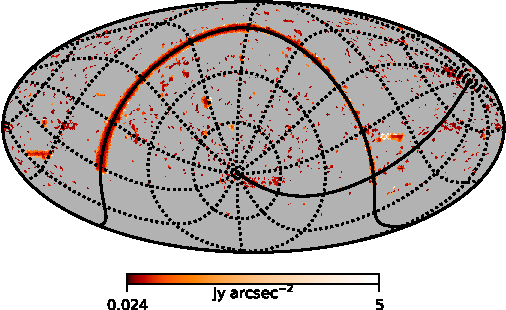
\includegraphics{mollweide-average-noise-galacticaxes-crop}
  \caption{All-sky noise map for this SCUBA-2 850\,\um{} legacy
    release. Each pixel represents the average noise across a single
    HEALPix tile. Tiles with fewer than 200 valid pixels were not
    included. The map is a cartesian Mollweide projection, with the
    axes of the galactic coordinate system overlain. The large curved
    stripe shows the extensive mapping of the Galactic Plane. Small points
    away from the plane predominantly represent daisy observations
    towards extragalactic sources scattered across the sky.}
  \label{fig:noise-mollweide}
\end{figure*}

This release includes individual reduced observations, co-adds of all
science observations that fell on a given tile, and catalogs of
extended regions and local peaks detected at
$>5\sigma$. Fig.\,\ref{fig:noise-mollweide} shows the all sky noise map
of the co-adds in this release, showing the average RMS across all
valid pixels in a tile as a single square.

All pointing and science observations from our time range were reduced
using the ORAC-DR recipe \texttt{REDUCE\_SCAN\_JSA\_PUBLIC} onto
HEALPix tiles (see Section \ref{sec:healpix}) using the HPX
projection, which leaves the observations fully reduced maps in units
of pW (see Section \ref{sec:dr}). The individual maps are available to
download through CADC/the JSA, where they will be listed under their
original project code and meta data. Pointing observations were not
used or analysed further in this data set.

All the reduced science observations were individually examined to
determine if they met our quality standards (see Section
\ref{sec:QA}). Co-adds were then made for every HEALPix tile with data
falling onto it, using the PICARD recipe \texttt{COADD\_JSA\_TILES}
(see Section \ref{sec:coadd}), producing a co-added tile calibrated in
units of m\jyas{} (for details on calibration see Section
\ref{sec:calib}). For every co-added tile, the PICARD recipe
\texttt{JSA\_CATALOGUE} was then run to produce (if detected) extent
and peak catalogues of detected emission (see Section
\ref{sec:cat}). See Fig.\,\ref{fig:flowchart} for an example of
the flow of data through these recipes.

\begin{figure}
  \centering
  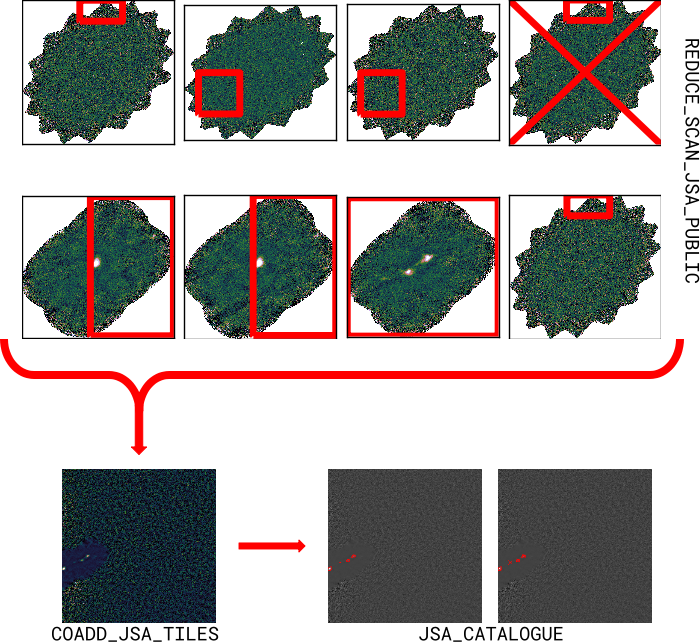
\includegraphics[width=1.0\linewidth]{flowchart}
  \caption{Flow chart indicating flow of observations through the
    system. Here, 8 of the input observations into tile 3311 are
    shown. Red boxes indicate the part of the observation that fell
    onto this tile. A red 'X' indicates an observation that was judged
    as 'BAD' during the Quality Assurance (QA) analysis. Captions
    indicate the ORAC-DR or PICARD recipe name that produces the output.}
  \label{fig:flowchart}
\end{figure}

\subsection{Included Observations}



This release includes publicly-released 850\,\um\ science observations
observed between 2011 February 2 and 2015 March 1, including
observations from calibration projects, PI projects, and the JCMT
Legacy Surveys (JLS). See \citealt{ChrysostomouJLS} for an overview of the
JCMT Legacy Survey program, which included: the Gould Belt Survey
\citep{GBS}, the SCUBA-2 ambitious Sky Survey \citep{SASSy}, the
Cosmology Legacy Survey \citep{Geach2013}, the JCMT Galactic Plane Survey
\citep{JPS}, the Nearby Galaxy Survey ??, and the Debris Disk Survey
\citep{SONS}.  The first block of these data, from 2011 to 2013 August 1
was previously reduced and publicly released in September 2015,
using the same configuration and co-add criteria as described in this
paper.
% add note -- available at (URL for download)
%\note{Has any NGLS SCUBA-2 data been published (NO)? Need need proper
%  SASSy refs. (There are none better as far as we know...)}


Observations from earlier than 2011 were not included, as these were
taken in \emph{shared risk} mode while instrument commissioning was
still being conducted, and the data from that era are more problematic
\citep{SC19,Dempsey2010}. Pointing observations, and science
observations from within the appropriate time period which failed QA
were still reduced using this standardised configuration\footnote{and
  are available for interested parties to download from the JSA}, but
have not been included in the co-added products (see \sref{sec:QA} for
more detail on this).

The observations included in this release were each taken in one of
the two different SCUBA-2 standard scan patterns: CV\_DAISY, a
fixed-size scan pattern used for covering small areas, and CURVY\_PONG
patterns at various user chosen sizes. The scanning speed is not the
same between these scan patterns, and there will be some inconsistency
in the size scales as SCUBA-2 reductions are sensitive to the
observing mode that was used. However, as our reduction has been
extremely conservative and has filtered out structure on scales larger
than 200\arcsec, we believe this effect should be minimized in our
co-adds.





\subsection{Overall statistics}
\begin{deluxetable}{lrrrrrr}
\tablecaption{Types of observation included in this
  release.\label{tab:typesobs}}
\tablecolumns{7}
\tablehead{
 & \multicolumn{3}{c}{Indiv. Obs} & \multicolumn{3}{c}{Coadds}\\
\cline{2-4}\cline{5-7}
\colhead{Type} & \multicolumn{1}{p{0.75cm}}{Num. obs.} & \multicolumn{1}{p{0.75cm}}{Time (hrs)} & \colhead{Tiles} & \multicolumn{1}{p{0.75cm}}{Num. obs.} & \multicolumn{1}{p{0.75cm}}{Time (hrs)} & \colhead{Tiles}}
\startdata
All & 21464 & 6420.0 & 4403 & 12404 & 5828.1 & 4151 \\
Sci & 12594 & 5914.5 & 4185 & 12404 & 5828.1 & 4151 \\
Point. & 8870 & 505.5 & 292 & 0 & 0.0 & 0 \\
Calib. & 2234 & 138.1 & 22 & 2200 & 135.9 & 22 \\
JLS & 6143 & 3642.2 & 2156 & 6023 & 3575.3 & 2145 \\
PI & 4217 & 2134.2 & 2329 & 4181 & 2117.0 & 2303\\
\enddata
\end{deluxetable}

In total, 21464 observations were reduced representing 6420 hours of
observing time, towards 4403 distinct HEALPix tiles. The co-added
observations include 12404 observations (5828 hours or 242.8 days)
towards 4154 tiles. These co-adds were made up of 136 hours of science
calibration observations, 3575 hours of data taken for the JCMT Legacy
Surveys and 2117 hours of data taken for PI projects. This information
is summarized in Table \ref{tab:typesobs}. The co-adds include 1.69
gigapixels of valid data, corresponding to ~1356 square
degrees.\footnote{\note{1.69e9 * (3.22/(60.0*60.0)**2?}}. For
comparison, the SCUBA Legacy Catalogue \citep{DiFrancesco2008} covered
19.6 square degrees in their  `Fundamental Map Data Set,
and 29.3 square degrees in their fuller `Extended Map Data Set'

  Source
detection was carried out on all of the co-added tiles, and this
detected emission in 1.37 square degrees (4.17e-4 steradians, or
0.33\% of the area observed.)



Because the observations used here are from a wide variety of projects
aiming for a variety of noise levels, our noise maps are extremely
heterogenous. Figure~\ref{fig:noise-mollweide} shows the all-sky
distribution of the noise maps of our
co-adds. Figure~\ref{fig:histonoise} shows a histogram of the noise in
each pixel of the co-added tiles. Table~\ref{tab:noises} shows the area
of our co-adds which has a noise level below various common
values. This is calculated by finding the number of pixels which have
a noise value less than or equal to a given limit. For convenience of
those readers most used to Jy\,beam\textsuperscript{$-1$}, we have
provided a very approximate equivalent flux density in those units by
dividing by our derived arcsecond Flux Conversion Factor (FCF)
(2.48\,\jyas\,pW$^{-2}$) and multiplying by the JCMT `standard' beam FCF
(537\,Jy\,beam$^{-1}$\,pW$^{-1}$. Please note that a beam FCF has not been
derived for this data set, so we do not recommend using this
calibration when extracting fluxes as a self-derived FCF would
probably have a systematic offset of a few percent from the `standard'
values (as shown for the arcsecond FCF in Section~\ref{sec:calib}).

\begin{deluxetable}{lDDD}
  \tablecaption{Areas of the release with an RMS noise less than or
    equal to the given value. \label{tab:noises}}
  \tablecolumns{4}
  \tablehead{%
%    \colhead{test} &
    \colhead{m\jyas{}}&
    \multicolumn{2}{p{1.5cm}}{Approx. mJy\,beam\textsuperscript{$-$1}}&
    \multicolumn{2}{p{1.25cm}}{\centering Area\linebreak(Sq.\,Deg.)}&
    \multicolumn{2}{p{1.25cm}}{\centering Area\linebreak(\%)}%
  }
  \startdata
  \decimals
   0.005 & 1.1 & 0.25 & 0.02 \\
  0.01 & 2.2 & 2.05 & 0.15 \\
  0.05 & 11 & 58.9 & 4.3 \\
   0.1 & 22 & 153.3 & 11 \\
   0.25 & 54 & 382.8  & 28 \\
   0.5 & 110 & 1128.6 & 83 \\
   1.0 & 220 & 1296.4 & 96 \\
  \enddata
\end{deluxetable}
\begin{figure}
  \centering
  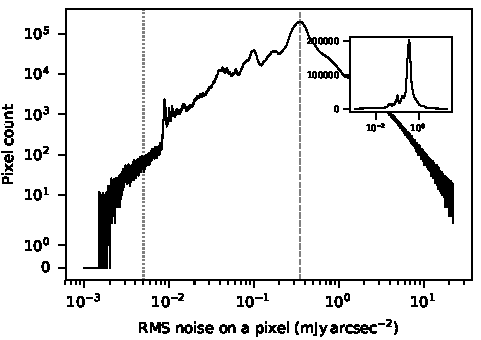
\includegraphics{coadds-noise-histogram.pdf}
  \caption{Histogram of the RMS noise on each pixel in the co-adds. The
    main plot is shown with a log y-axis scale, and a linear y-axis
    scale is shown in the inset. Note that no trimming of observations
    is done for this, so the noisy edges of the SCUBA-2 observing
    patterns are included. The noise is taken from the \texttt{makemap}
    produced variance array, which uses the scatter of input data
    points to estimate the variance of a given pixel while reducing
    the raw time series onto a sky map.}
  \label{fig:histonoise}
\end{figure}
\subsection{The deepest maps}
Twenty of our co-added tiles contain pixels with a noise better than
0.005\,m\jyas (corresponding to very roughly 1\,m\jybm). These include
our three most common standard JCMT SCUBA-2 calibrators (CRL 618, CRL
2688 and Arp 220), and several deep cosmology fields that were
observed by the JCMT Cosmology Legacy Survey and various PI
projects. For reference, these twenty tiles, along with some
statistics of their deep regions are listed in
Table\,\ref{tab:deepmaps}.
%mention that examination by eye of these tiles shows the noise to be reasonable?

%\floattable
\begin{deluxetable}{rc r c c p{2cm}}
  \tablecaption{The twenty co-added tiles which contain regions with a
    noise at or better than 0.005\,m\jyas.\label{tab:deepmaps} }

\tabletypesize{\scriptsize}
\tablehead{
\colhead{Tile} & \colhead{Area} &
\colhead{Num.} &
\colhead{exp. time} &
\colhead{Av. RMS} &
\colhead{Source}\\
\colhead{} & \colhead{Sq. Deg.} &
\colhead{Pixels} &
\colhead{hrs\,pixel$^{-1}$} &
\colhead{m\jyas} &
\colhead{names}
}
\startdata
9831 &  0.0010 & 1303 & 1.88 & 4.9E-03 & CL1604+4304\\
8921 &  0.0026 & 3207 & 3.36 & 4.6E-03 & MACS J1423.8+2404\\
8915 &  0.0003 & 341 & 2.99 & 4.8E-03 & MACS J1423.8+2404\\
8673 &  0.0017 & 2069 & 3.65 & 4.7E-03 & Arp220\\
17679 &  0.0017 & 2087 & 3.22 & 4.2E-03 & UKIDSS-UDS-CANDELS\\
12640 &  0.0029 & 3640 & 3.04 & 4.6E-03 & MACSJ2153.6+1741, Abell 2390\\
1244 &  0.0023 & 2893 & 5.17 & 4.4E-03 & CRL618\\
1238 &  0.0024 & 2956 & 5.19 & 4.4E-03 & CRL618\\
11596 &  0.0016 & 2036 & 3.04 & 4.8E-03 & Q1700\\
28448 &  0.0057 & 7143 & 3.10 & 4.4E-03 & MACS J1149.5+2223\\
26189 &  0.0084 & 10471 & 2.85 & 4.4E-03 & Abell 1689\\
17741 &  0.0066 & 8275 & 4.06 & 4.4E-03 & Abell 370\\
13297 &  0.0068 & 8440 & 4.67 & 4.4E-03 & CRL2688\\
12642 &  0.0153 & 19104 & 3.97 & 4.2E-03 & MACSJ2153.6+1741, Abell 2390\\
6383 &  0.0216 & 26955 & 3.96 & 4.1E-03 & MACSJ0717.5+3745\\
35935 &  0.0185 & 23106 & 4.91 & 4.2E-03 & CDF-S\\
17690 &  0.0307 & 38318 & 5.24 & 3.5E-03 & UKIDSS-UDS-CANDELS\\
11425 &  0.0349 & 43614 & 5.90 & 3.3E-03 & AEGIS-CANDELS\\
11252 &  0.0352 & 43943 & 6.47 & 3.4E-03 & GOODS-N-CANDELS, CDF-N\\
27258 &  0.0505 & 63077 & 9.20 & 2.8E-03 & COSMOS-CANDELS\\
\enddata
\tablecomments{This table lists the tile numbers, representative
  source names (based on the names chosen by the projects whose data
  is included). It also lists some statistics calculated on the set of
  pixels in each tile which have an RMS $\leq$0.05m\jyas: the area, the
  number of pixels, the average exposure time per pixel and the mean
  noise across these pixels. The deepest tile in this list, 27258, is
  also shown in Figure \ref{fig:t27258}.}\end{deluxetable}
% \begin{table}
% \centering
% \begin{tabular}{l c r l}
%   \hline
%   Jy/arcsec$^{2}$& mJy/beam  & \multicolumn{2}{c}{Area}\\
%                 &          &  Sq. Deg. & Percent. \\
%   \hline
%   1  & 229.5& 740.7 & 94\% \\
%   0.5  & 114.7& 585.4 & 74\% \\
%   0.25  & 57.4& 246.0 & 31\%\\
%   0.1 & 22.9& 71.8 & 9.0\%\\
%   0.05 & 11.5& 37.0 & 4.7\%\\
% %  0.01 &2.3 & 0.5 & $<$0.1\%\\
%   \hline
% \end{tabular}
% \caption{Areas of the release which have an RMS noise less than or
%   equal to the given value. \label{tab:noises} }
% \end{table}
%\subsection{Comparison with the SCUBA Legacy Catalogue}
\section{Example regions}
This data release includes emission towards objects covering the full
diversity of non-solar system structures observed by the JCMT --
including dusty disks, complex filamentary molecular clouds, nearby
galaxies, extragalactic point sources and extremely deep surveys of
standard cosmological fields. Although providing full examples of all
types of emisison is beyond the scope of this paper, we here present
some of our co-added tiles covering a range of source types.

\subsection{G034.27+0.15}
The source G034.27+0.15 is a bright, high-mass star-forming region
that has been observed in a wide variety of
wavelengths. Figure~\ref{fig:g34-3} shows our co-added tile, noise map,
extent catalogue and peak catalogue towards this source. This co-add
includes data primarily from JCMT calibration projects of this source,
but also two observations from a University of Hawaii (UH) PI project
(M13AH07B).\note{Was this published?}. The noise maps for this co-add
shows the characteristic 'CV\_DAISY' scan pattern towards the central
source, with two overlapping small PONG observations covering a wider
extent. This field also illustrates the artificially high noise we
see towards bright sources (see Section~\ref{sec:dr}) -- this is seen
in the higher noise points towards the central source and the bright
points in the filament extending towards the top left. Examination of
the extent and peak catalogues, however, (shown below) indicates that
this problem did not prevent a detection of the emission in these
regions. Our experience has been that these high-noise areas only
occur towards bright regions, so they are still clearly detected in
our extent catalogs, with an signal-to-noise ratio (SNR) of $>5$.



% includes a variety of types of structure three examples shown here
% to examine the co-adds and the catalogs.  Includes: filamentary
% region (G34.3), bright point source (CRL618, a standard calibrator)
% and the deepest map in our data set, a long observation of what is a
% 'blank field in any single observation, but reveals a multitude of
% deep submm galaxies when co-added.


\begin{figure*}
  \centering
  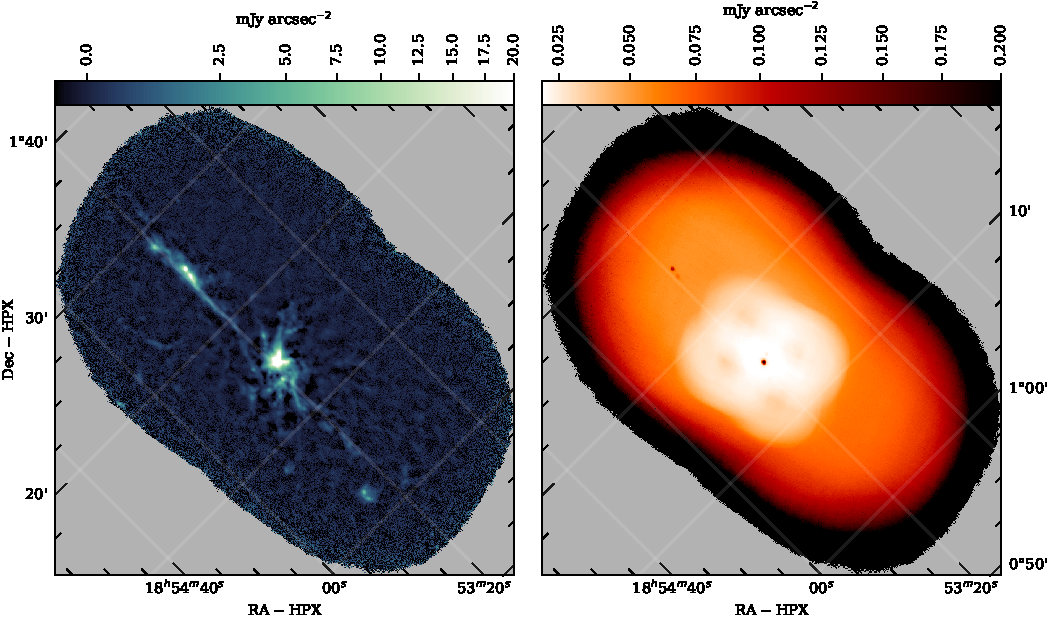
\includegraphics{tile30318-g34-coadd-noise.pdf}
  \\[3mm]
  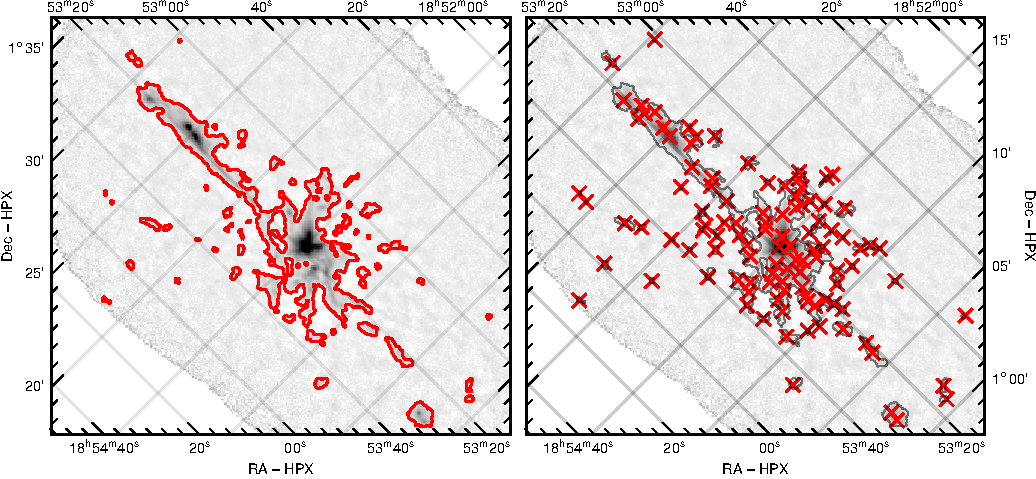
\includegraphics{tile30318-g34-extent-peak.pdf}
  \caption{Examples of the co-add, noise map, extent catalogue and peak
    catalogue towards tile 30318 containing the high-mass star-forming
    source G034.27+0.15}
  \label{fig:g34-3}
\end{figure*}
\subsection{CRL\,618}
CRL 618 is one of the JCMT's standard flux calibration sources for
SCUBA-2 observing. As such, this co-add includes 923 observations using
51 hours of observing time across the small CV\_DAISY area, shown in
Figure~\ref{fig:crl618}. We achieved an extremely high noise due to
this large number of repeats -- achieving a noise better than
0.005\,m\jyas\ around the central source. A zoom in on the central
sources shows clearly a variety of point sources detected in this deep
co-add. In addition, it can readily be seen by eye that there appear to
be additional sources that are missed by our cataloging procedure due
to the negative bowling around the very bright source. Horizontal and
vertical cut throughs are shown to help visualise this bowling.

\begin{figure*}
  \centering
  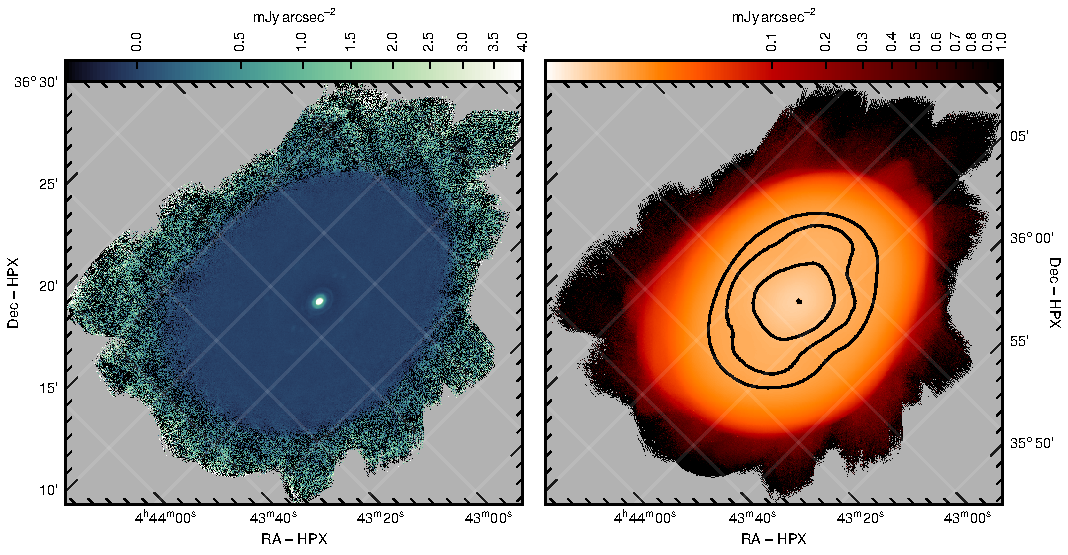
\includegraphics{crl618-whole-map.pdf}
  \\[3mm]
  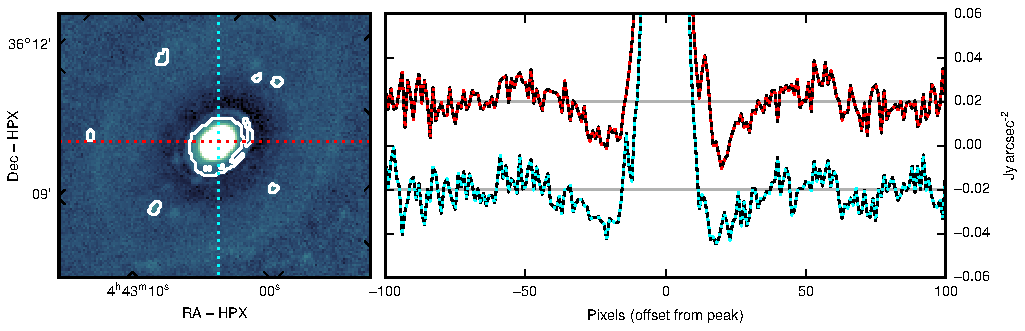
\includegraphics{crl618-sourceonly.pdf}
  \caption{Examples of the co-add, noise map, and extents towards the
    standard calibration source CRL 618, consisting of tiles 1238 and
    1244. This co-add contains data from XX900 observations (XXhrs
    elapsed observing time). The contours on the noise map indicate
    the 0.005, 0.006 and 0.007 m\jyas\ noise contours. On the bottom
    row a zoom in of the central source showing the detected extents
    around the source is shown (Left), as well as horizontal and
    vertical cuts through the peak (Right). In these cut throughs the
    ~0.01 m\jyas\ bowling around the bright central source can be
    easily seen. }
  \label{fig:crl618}
\end{figure*}

\subsection{Tile 27258: Deep COSMOS-CANDELS field}
Here we present our deepest map. This includes data both from the JCMT
Cosmology Legacy Survey \citep[recently published in][]{Geach2016} but
also from various University of Hawaii deep surveys
\citep{Casey2013,Chen2013,Chen2013a}. By being able to include
publicly available data taken by different projects we can achieve a
deeper map than possible with only one data set. Our co-add includes
both wide PONG observations, and very deep DAISY
observations. Figure~\ref{fig:t27258} shows both the entire tile, its
noise map, and also a zoom in of the deepest region. In the noise map
it is possible to see the imprint of the various scan patterns. Note
that we do not appear to have problems with addition of the high noise
edges, indicating that our variance arrays are reasonably accurate
even in these higher noise areas.

In this deep map, it can clearly be seen that there are point sources
spread across the full map. Although for optimal detection of point
sources a beam matched filter should be used, even without using that
we detect a large number of these objects. Figure~\ref{fig:27258}
shows a comparison of our detections, the CLS's detections from their
first data release \citep{Geach2016} and those of
\citet{Casey2013}. Although these three methods do not detect exactly the
same objects, there are many correspondances between them.

\begin{figure*}
  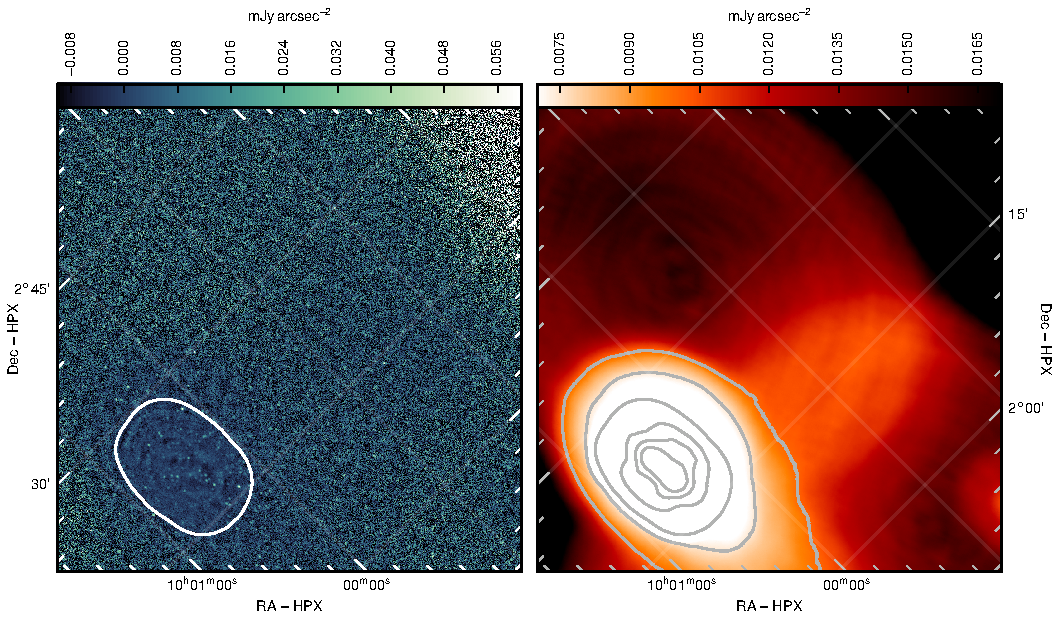
\includegraphics{27258-whole-map.pdf}
  \\[3mm]
  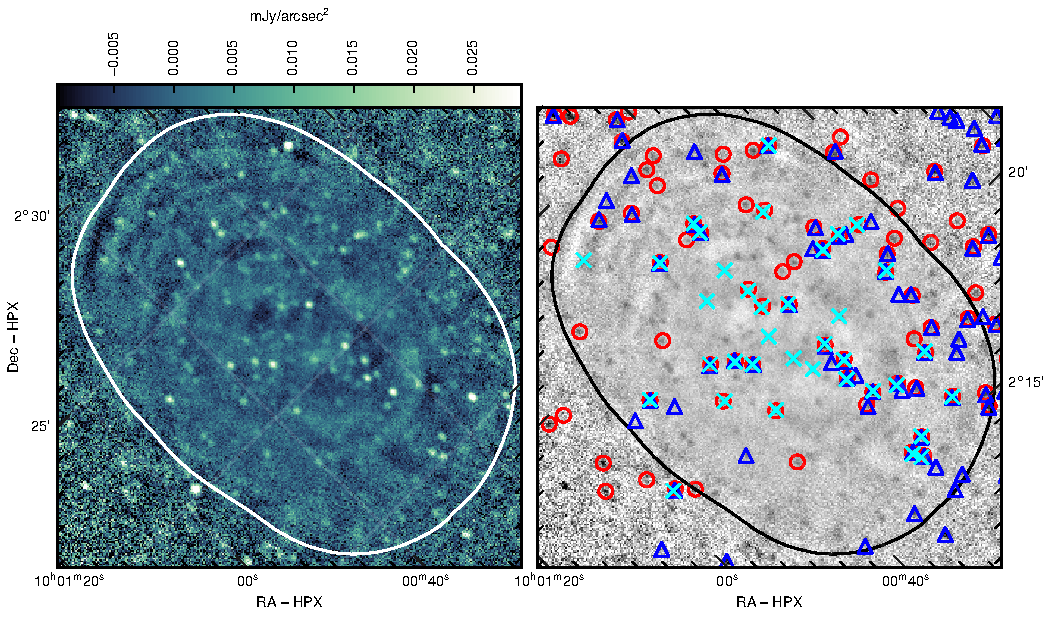
\includegraphics{27258-zoomin.pdf}
  \caption{Tile 27258 showing an extrememly deep co-add towards a
    COSMOS field. This tile pongs and daisy observations taken by JCMT
    Cosmology Legacy survey and several UH cosmoloy projects. Parts of
    these data were published in
    \citet{Casey2013,Chen2013,Chen2013a,Geach2016}. Top Left: emission
    map of the entire co-added tile. Note the deep daisy seen in the
    bottom right. Top right: noise map of the entire tile. Contours
    indicate the 1.75, 2, 2.5, 5, 7.5, and 10 m\jyas\ regions. Bottom
    left: an enlargement of the deepest region of the map, showing the
    850\micron\ data. The contour indicates the < 5m\jyas\ noise
    region. Bottom right: comparison of the source catalogues produced
    here (shown as cyan crosses), as published in \citealt{Casey2013}
    (red circles) and as found by the JCMT CLS 850um DR1 \citep[blue
    triangles]{Geach2016}. }
  \label{fig:t27258}
\end{figure*}


\section{SCUBA-2 data reduction}
\label{sec:dr}
SCUBA-2 observations are reduced using the Starlink SMURF program
\texttt{makemap}. In brief, this is an iterative process that divides
the data set into various instrumental and astronomical signals. There
is an extremely large number of user-adjustable parameters that can
affect the final map, depending on the science goals of the users and
the structure of the astronomical emission observed. \note{For example, a
cosmologist interested in detecting only faint point sources in a
primarily blank map would use a distinctly different set of parameters
from a galactic astronomer looking at bright, extended and
structurally complex emission.} For full details on the SCUBA-2 map
maker, please see \citet{Chapin2013}.


%Redraft this paragraph -- more paper-esque.
To guide astronomical users, the JCMT-supported Starlink software
comes with a series of standard configuration files for a variety of
common science cases.
% Although all JCMT observations are run through an automated pipeline
% every night \citep{2011scuba2dr,2015oracdr}, these reductions rely
% on the PI of the project selecting an appropriate reduction `recipe'
% for their science goals.
These standard configuration files can produce very poor results when
used on an inappropriate observation -- for example, the standard
SCUBA-2 configuration file used for calibrator observations is tuned
to expect a bright, compact source at the centre of the map. If used
by mistake on a blank field this recipe could easily create \emph{fake
  emission} in the form of large bloom-like structures. Avoiding this
sort of error was the paramount consideration when selecting the
configuration parameters.

Given the nature of SCUBA-2 data reduction algorithms, the main focus
in developing this \emph{legacy} configuration was on maximising the
confidence that could be placed in detection of emission, at the
expense of not attempting to recover large scale structures.

These observations were reduced using Starlink, Starjava and ORAC-DR
software developed between versions 2014A and 2015A. Interested
parties seeking to replicate these results can do so by checking out
the version of the code tagged as `2015A-legacy' release in the
Starlink code repositories\footnote{(See
  https://github.com/Starlink/starlink,
  https://github.com/Starlink/starjava and
  https://github.com/Starlink/ORAC-DR).}.


\subsection{Details of our chosen configuration file}

\note{Harriet suggests we might want an additional appendix, and the
  following sentence in this paragraph ``An expanded explanation of
  the SCUBA-2 mapmaker and its advances since Chapin et al. 2013 can
  be found in Appendix B." with additional information in an
  appendix'').}



For the exact configuration file used in the legacy reduction see
Appendix~\ref{app:config}. In this particular reduction, after the initial
pre-processing stage, the SCUBA-2 mapmaker recipe performs five
iterations in which the astronomical signal is retained rather than
being removed (as in a normal iteration) prior to starting the next
iteration (specified using \texttt{ast.skip=5}). These initial
iterations allow the reduction process to focus on creating a mask
that identifies any unusually bright region. This is useful since such
regions may cause ringing in subsequent estimates of the low-frequency
noise in each bolometer. During these iterations ``bright'' pixels are
taken to be those with a signal-to-noise ratio greater than 5.0, plus
any other pixels that are attached contiguously to such pixels down
the an SNR of 3 (specified by using \texttt{flt.zero\_snr=5} and
\texttt{flt.zero\_snrlo=3}).

During all iterations an atmospheric correction is applied and data
are filtered to remove any features on scales larger than 200". In
addition to this a separate common mode model is produced for each
subarray (specified with \texttt{com.perarray=1}). Having a separate
common mode estimate per subarray prevents artificial flux (also
known as ``fake blooms'') being introduced into the map where the
common modes vary significantly and are not well represented by a
single common mode. The disadvantage with having a separate common
mode for each subarray is that the reduction is limited to recovering
emission structures that are on the same scale or less than the
subarray size (approximately 200").

After the initial five iterations the recipe then performs up to 20
further iterations with all the models (specified by
\texttt{numiter=-25}; the initial five iterations plus these additional 20
iterations containing all models). Each of these remaining iterations
removes the astronomical signal from the residuals prior to starting
the next iteration. However, to prevent instabilities in the iterative
process, this subtraction only occurs within regions corresponding to
bright sources.  The mask identifying such sources is creating in the
same way as the mask used by the low-frequency noise filter (``FLT''
model): source pixels are taken to be those with a signal-to-noise
ratio greater than 5.0 (plus any other pixels that are attached
contiguously to such pixels down to an SNR of 3 (specified by using
\texttt{ast.zero\_snr=5} and \texttt{ast.zero\_snrlo=3}).

The map maker exits before the 20th iteration if the \texttt{maptol}
parameter --- the change between maps --- has reached a mean value of 1\%
of the noise level (specified by \texttt{maptol=0.01}).


% See Appendix~\ref{app:config} for the full configuration file. Some of
% the most important details are described below:

% Our mapmaker configuration first of all performs five iterations without
% creating an astronomical model of the source. \note{Harriet\&DSB: do
%   we have a short explanation of do we do this again?}. It will then
% perform up to 20 further iterations with all the models, but will exit
% before that point if the 'maptol' parameter has reached a mean value
% of 0.01.

% In order to decrease the production of fake 'blooms' of emission in
% the final map, we produce a separate COMMON mode model for each
% subarray (\texttt{com.perarray=1}). While this produces more reliable
% output (appropriate for this project which has comparatively minimal
% by eye checking of data), it has the effect of removing structure
% scales that are larger than the subarray size.

% \note{zero snr and zero snrlo: need a proper explanation for these}
% We also set the 'AST' and 'FLT' zero\_snr and zero\_snrlo values.

%Figure ?? shows a reduction of a single
%observation towards a standard calibrator, reduced using both the
%legacy configuration file presented here (in an HPX projection), and
%with the standard calibration reduction configuration `bright compact'
%on the tangent plane projection.

% \begin{figure}
%   \centering
%   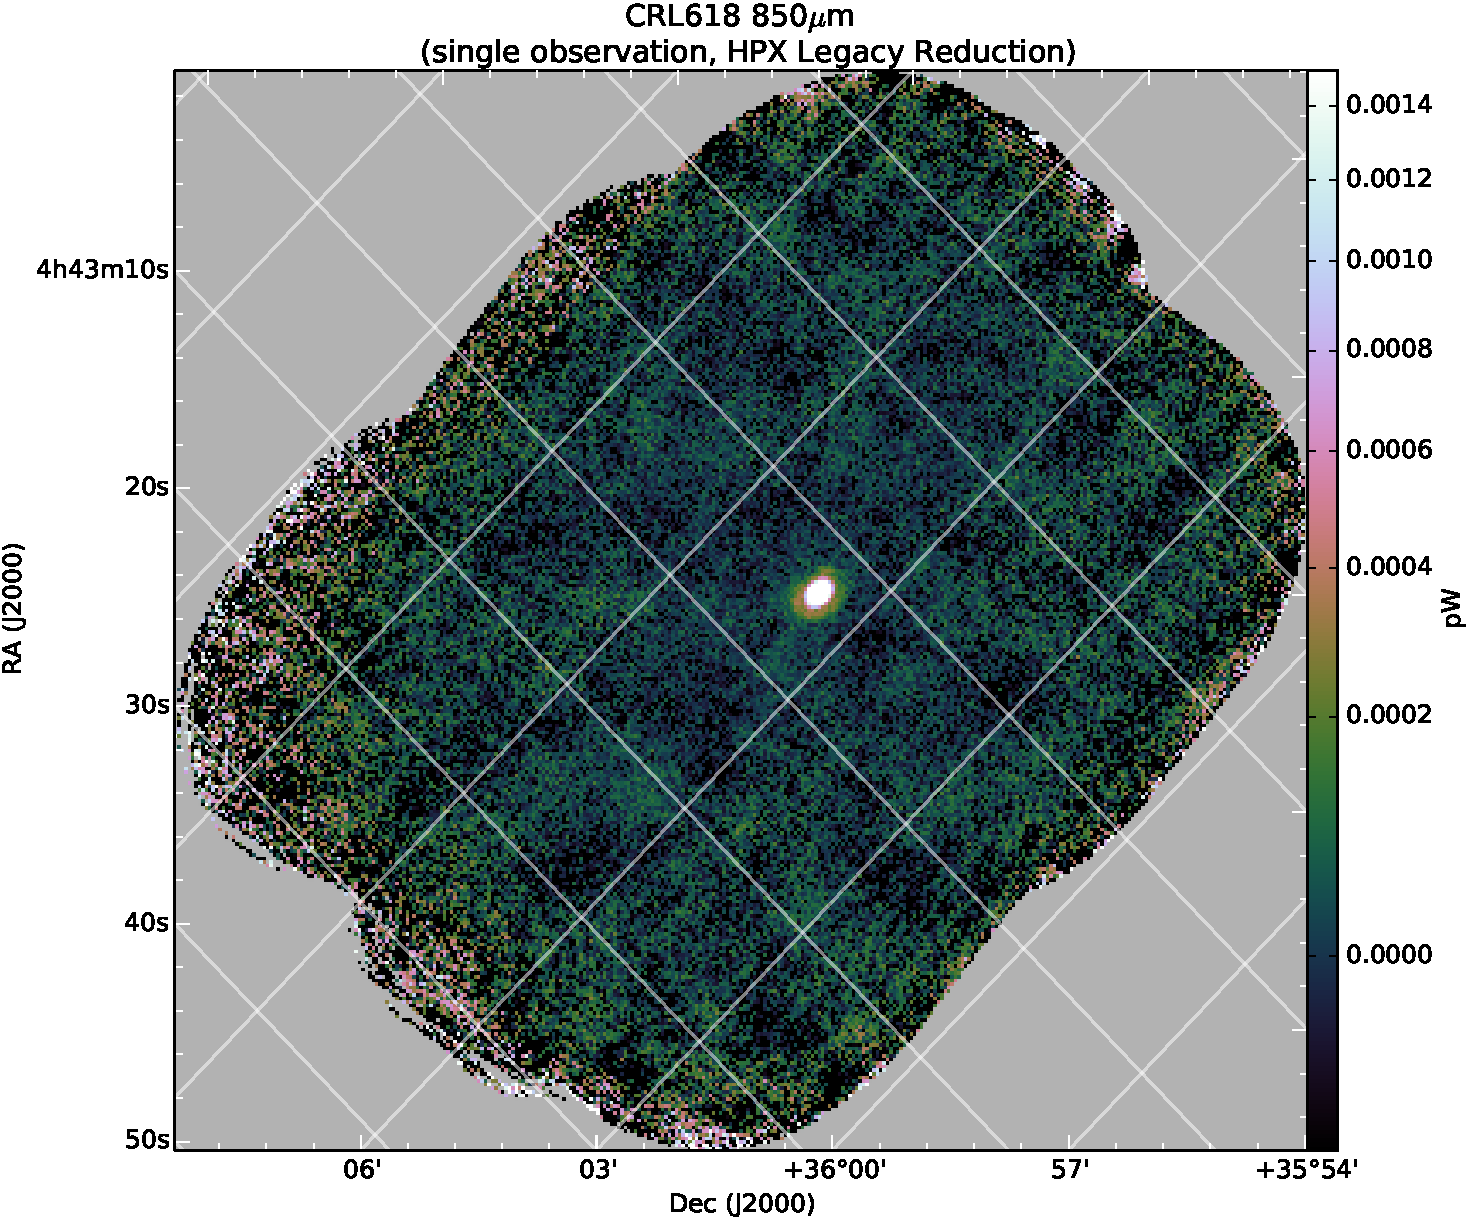
\includegraphics[width=0.45\linewidth]{crl618_example_legacyred}
%   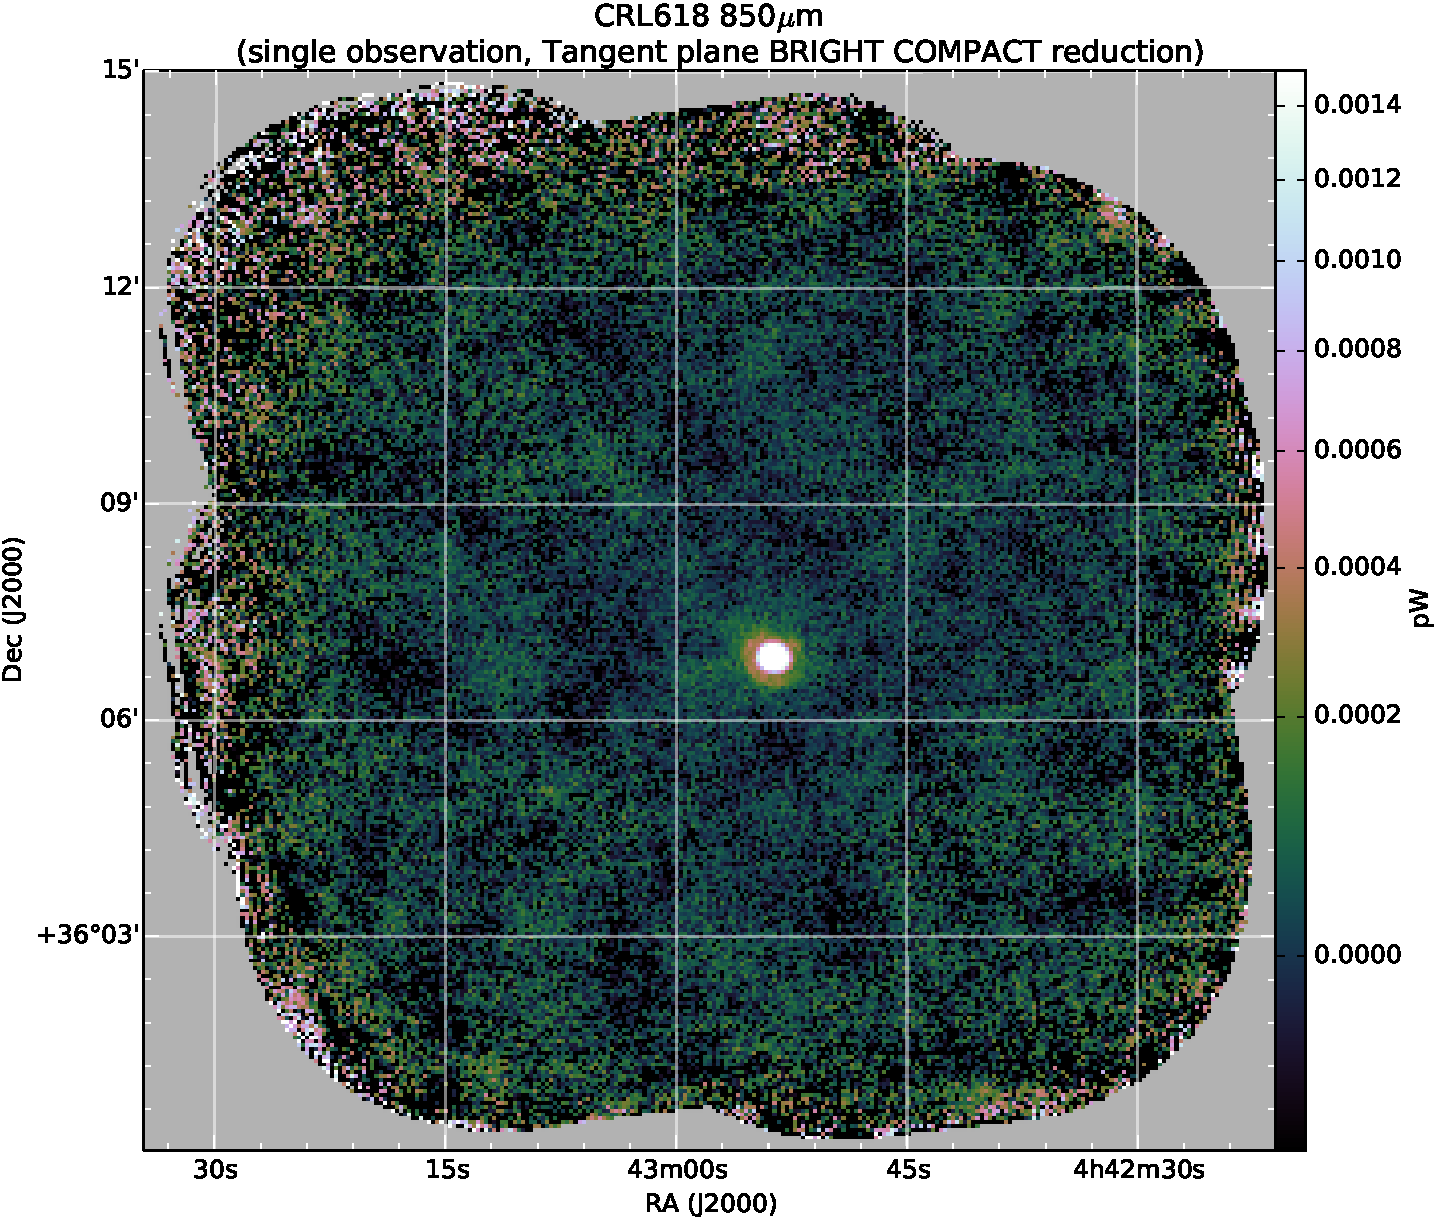
\includegraphics[width=0.45\linewidth]{crl618_example_bcred}
%   \caption{Left: A legacy 850\,\um{} reduction of a single observation
%     towards the JCMT standard calibration source CRL 618. Note that
%     the pixel axes are at 45 degrees to the RA and Dec axes. As each
%     pixel in the map is truly shaped like a diamond (i.e. a stretched
%     square), the distortion introduced by an image viewer that
%     displays every pixel as a square causes the source to appear
%     ellipsoidal. Right: For comparison, a standard non-HEALPix tangent
%     plane reduction with the Bright Compact configuration is shown for
%     the same source. Here the source appears more circular. Both maps
%     are shown in uncalibrated units of pW on the same scale. These
%     maps cover two tiles.}
%   \label{fig:crl618-example}
% \end{figure}


%Figure ?? shows a reduction of a single
%observation towards the complex, bright and extended OMC-1
%region. \todo{ Should this have a comparison with e.g. a GBS
%  reduction of this region, to show the difference in size scales?
%Or leave that for later}.

% \begin{figure}
%   \centering
%   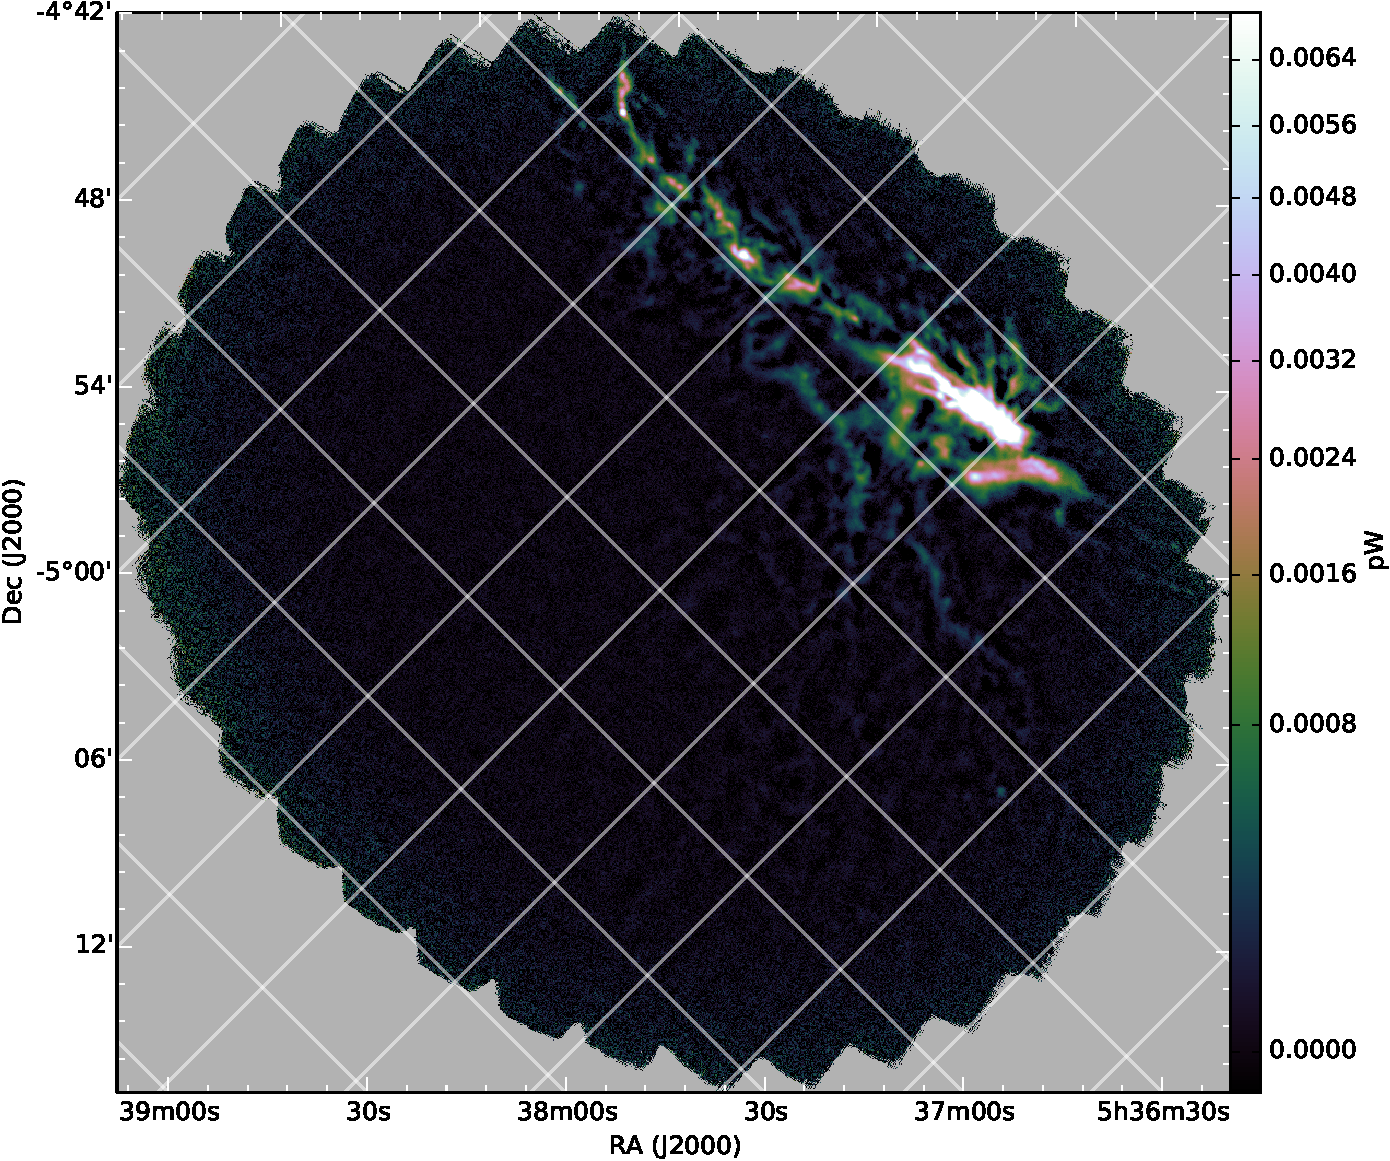
\includegraphics[width=0.6\linewidth]{omc1_example_legacy}
%   \caption{A legacy 850\,\um{} reduction of a single
%     observation(observation 93 from 2012-08-17) towards the OMC-1
%     source. This observation overlapped with three tiles: 22805, 21439 and
%     21438. }
%   \label{fig:omc1-example}
%     \end{figure}


\subsection{Co-adding of tiles}
\label{sec:coadd}
All non-pointing observations towards a given tile that passed QA were
co-added and calibrated using the PICARD recipe
\texttt{JSA\_CATALOGUE}. This uses \texttt{makemos} applications from
Starlink's \texttt{ccdpack} \citep[][\ascl{1403.021}]{SUN139}. This
co-adding was carried out as a variance-weighted mean. No despiking
was performed, and no clipping of the noisy edges of observations was
done; no evidence was seen that these were required. The variance map
for the co-added tile is also produced. The calibration from pW into
m\jyas\ was done by multiplying with an FCF of
2.48$\times$10\textsuperscript{3}\,m\jyas\,pW\textsuperscript{$-$1},
derived from our own data set -- see Section \ref{sec:calib}.

\subsection{Source Recovery}
Recently, work by \citet{Mairs2015} examined the recovery of sources
found inside and outside the \texttt{makemap} AST mask, specifically comparing
the JCMT Gould Belt Survey's reductions with the Legacy Release configuration
described here. They found that in SCUBA-2 reductions there is a
significant difference between recovery of sources inside and outside
the AST mask. Sources that are outside the AST-masked regions can have
their flux considerably under-represented. The AST masked region can be
thought of as approximately the region containing detectable emission,
using `detection' limits set in the specific configuration parameters
chosen. The effect is dependent on the size of the source -- extended
sources outside of the masked regions are poorly recovered in this
reduction, where as point sources are recovered well.  This issue does
in theory affect all reductions, including those using external masks
defined from previous knowledge of the emission, but is of course most
problematic for reductions such as these where the AST mask is defined
based only on detected emission from a single observation.

If users of this release are concerned about the recovery of specific
sources, each individual reduced observation contains a QUALITY array,
which indicating which areas of the map were and were not included in
the AST mask (and also the FLT mask).


\subsection{Size Scales}
We have excluded sizes scales larger than the subarray size from our
reduction. In addition, we have used a fairly aggressive large scale
filtering removing scales larger than 200 arcseconds.

\todo{Do we want some power spectra of this? not sure if they'd be very illuminating.}

\subsection{Negative Bowling}
Within the co-added maps of this release, negative bowling can be
clearly seen around bright sources. Figure~\ref{fig:crl618} shows this
clearly around the bright calibrator CRL\,618. The cut throughs in the
vertical and horizontal direction through the source show the bowling
at ~0.01\,m\jyas. No processing was done to try and ameliorate these
effects, and there will be significant loss of detected emission and
missing of entire sources in the emission catalogs, due to these
artificial negative regions around bright sources.

\todo{Do we need more examples of this? Find a good description of why
  this happens, should be in S2 cookbook somewhere.}

% \section{Comparison with legacy surveys}

% \todo{A SCUBA-2 image from each survey alongside a Legacy Release
%   version. Which wavelengths? SASSy only has one published field
%   \citep{MacKenzie2011}. JPS and NGLS may not have any yet. GBS has a
%   few recent papers with \citet{Rumble2015} published for Serpens.}


%\todo{Picture of a co-added tile? Both data and noise. Pick something
%with Daisy and pongs in it, as a comparison.}


%\todo{Each observation is gridded into pre-defined tiles. Are they
%  extinction corrected at that point? Unlike HARP processing
%  \citep{2015ACSISDR}, observations can be reduced independently and
%  then co-added. Extinction correction can be applied during co-adding
%  phase? How well are edge-effects handled by variance weighting?}
\section{Catalogues}
\label{sec:cat}
The JCMT Legacy release includes emission catalogues generated from
each of the co-added maps. As we have an extremely diverse set of
astronomical regions (including blank fields, point sources and large,
complex extended structures), we did not feel it would be possible to
perform specific astronomical source finding and
classification. Instead, this release focused on identifying first of
all \emph{regions of contiguous emission}, discussed here as
\emph{extents}, and secondly on \emph{identifying local maxima within
  those regions}, described here as \emph{peaks}. The primary goal of
these catalogues is to provide astronomers with regions of securely
detected emission.


We have chosen to use the Fellwalker algorithm \citep{Berry2015}, as
implemented in the Starlink CUPID \citep{cupid} package for this
analysis. Unlike the more commonly used ClumpFind which simply lays
discrete contour levels on the map and uses those to identify regions,
Fellwalker follows lines of ascent within the map to identify all
peaks of emission. We have found it to be robust and
easy-to-understand, and to produce intelligible results.

\subsection{Extents}
\label{sec:extents}
We have identified the regions of contiguous extended emission within
each tile by looking at the signal-to-noise maps of the co-added
tiles. We determined that we would consider all regions of contiguous
emission containing flux brighter than 5-$\sigma$ to be a single `extent'
for purposes of our reductions, if the region is larger in area than a
beam.  Here, a simple approximation of the beam was used (all sources
larger than 9 pixels). We followed the emission down to a noise level
of 3-$\sigma$. We considered using a more complex approach, but noise
spikes in \texttt{makemap} maps did not appear to be commonly falsely detected
with this approach. The main source of false detections in our
reductions would have been the previously discussed problem of `false
blooms of emission' occasionally produced by \texttt{makemap} reductions, if we
had not used a by-eye approach for flagging the handful of problematic
reductions and removing them from the co-adds.

The reduced observations, produced by SMURF's \texttt{makemap} routine, all
contain a variance array giving the noise towards each pixel, based on
the scatter of input data points to that pixel. Pixels with too small
a number of inputs to calculate a variance point are not included in
the individual maps. Our co-adding procedure uses this variance to
weight the input observations. We do see anomalously high noise
towards the center of bright sources \note{TODO: explain why!} (see
Fig.~\ref{fig:g34-3} for an example of this); however this is not at a
level to prevent a signal-to-noise 5-$\sigma$ detection.

\todo{Is this needed:? Note on varying noise within tiles -- show some examples,
  explaining why its so necessary to use SNR instead of a
  representative noise when the noise varies across the tile.}

We used the Fellwalker algorithm as implemented in CUPID on an SNR map
to produce contiguous regions of emission and to identify the position
of the peak pixel within each map, and these outlines are available
both as a FITS format mask file, as a HEALPix Multi-Order-Coverage
file (MOC) and as a rough approximation by STC-S polygon. The
catalogue for each tile indicates the ID of the clump, the RA and Dec
of the peak pixel, the total flux contained within the entire extent,
the flux of the peak pixel, and the area of the entire extent. The
catalog also includes the approximation of the outline of the extent
as an STC-S polygon string. An excerpt from the extent catalog for
Tile 30318 (containing G34.3) is shown in Table~\ref{tab:extents}.







\subsection{Peaks}
\label{sec:peaks}
In order to provide some information about the nature of emission
within the extents, this release includes identification of local
maxima within the extents. \emph{It is important to note that these
  should not in general be considered as point sources.} We identified
these points by running the Fellwalker algorithm (from Cupid) on the
extent map. The peak detections were not created from the SNR map, as
we could assume by only looking within the detected extents that we
were already looking at detected emission.

As our maps contain a varying noise, we used the mean noise across the
entire detected extent as a representative noise. We then used the
Fellwalker algorithm with that noise as the RMS value, and identified
as individual local maxima those which contained a peak of 5-$\sigma$,
followed down to a noise level of 3-$\sigma$, and with at least a
5-$\sigma$ dip between them and neighbouring maxima. Our output
catalogue contains the ID of the peak, the RA and Dec of the peak
pixel, the flux in the peak pixel, and the ID of the extent the peak
was drawn from. An excerpt from the peak catalog for Tile 30318 is
shown in Table~\ref{tab:peaks}.

We decided not to include the outlines of all emission counted as
being within that object or clump, as we felt that would encourage
users to consider the peaks as being real, physical objects. Although
they may be in some cases, in many other cases the peak is simply a
local maxima within a complex molecular cloud. The `clump outlines'
produced by software such as CUPID always reflect the arbitrarily
chosen boundaries of dips and minimum heights, and should not be
assumed to represent physical objects without considerable further
modelling.

(\todo{Does this need further discussion? Cite various issue with clumpfind papers maybe?}.)


\section{HEALPix grid}
\label{sec:healpix}

To produce a uniform reduction of all public data, it is necessary to
have a suitable scheme for dividing the sky into pre-determined tiles
and pixels to grid the data onto.  The scheme needed to be well
defined in advance, without reference to the position of existing
observations, for consistency and in order to be able to easily
incorporate further data as they become public.  The tiling scheme
which was chosen is that offered by HEALPix \citep[Hierarchical Equal
Area isoLatitude Pixelization,][]{Gorski2005}, commonly used by
cosmologists. The HEALPix system starts by dividing the sky into
twelve facets, and then recursively divides these cells in four at each
higher resolution level.  There are two standard numbering schemes
used with HEALPix, of which the ``nested'' scheme has been used to
label tiles in this release, for convenience with the HPX projection
and compatibility with Virtual Observatory systems such as MOC
\citep[Multi-Order Coverage,][]{2013ASPC..475..135F}.

Pixels within the individual tiles also use the HEALPix grid, which
ensures that the pixelization is continous between each tile and the
adjacent tiles.  This has the advantage that the tiles can be joined
simply by abutting them.  This is done via the HPX projection
\citep{Calabretta2007} which allows the the HEALPix grid to be used
for conventional 2D FITS images.

While HEALPix has the advantage that all pixels have the same area,
the trade off is that the pixels are not all square: they can vary in
width and height while maintaining the constant area.  There are also
discontinuities in the angle of the grid lines at some facet
boundaries.  This is largely a display problem, as although image
viewers with a modern WCS implementation can handle files in the HPX
projection, the grid lines, and therefore astronomical sources also,
will appear bent at these positions.\footnote{If you are concerned by
  the visual appearance of HEALPix maps in your display and wish to
  reassure yourself that any apparent distortion is only due to
  display issues in your image viewer, we would recommend verifying
  the shape and position by contouring the map over a tangent-plane
  map.}


\begin{table}
\caption{HEALPix parameters used in this release.  \label{tab:hpxpar}}
\centering
\begin{tabular}{rl}
\tableline
Tile size & $\sim$ 1\degr square \\
Tile $N_\mathrm{side}$ & 64 \\
Pixels in a tile  & 1024 $\times$ 1024\\
Pixel area &  3.22$^{2}$ square arcseconds\\
Pixel $N_\mathrm{side}$ & $2^{16}$ \\
\tableline
\end{tabular}
\end{table}


%\footnote{To re-grid one or more HEALPix tiles onto a standard RA-Dec
%  projection, the Starlink \textsc{smurf} command \texttt{jsajoin} can
%  be used \citep[][\ascl{1310.007}]{SUN258}.}

\section{QA}
\label{sec:QA}

% \subsection{Standard JCMT QA States}
% All observations taken by the JCMT are classified as \status{GOOD}
% (the default), \status{BAD}, \status{QUESTIONABLE}, \status{JUNK} or
% \status{REJECTED}. We included \status{GOOD}, \status{QUESTIONABLE}
% and \status{REJECTED} data in our co-adds. The \status{REJECTED} state
% is used by the JLS teams to indicate that a particular observation did
% not meet their particular QA criterion but the data are otherwise
% usable. The \status{QUESTIONABLE} state was originally designed to be
% a transient state that would be resolved into either \status{BAD} or
% \status{GOOD} after analysis, but in practical terms there was not a
% workflow to ensure this, so some observations have this flag in the
% archive.

% Usually (in the standard nightly reduction pipelines)
% \status{QUESTIONABLE} data is treated as if it is \status{BAD} for the
% purposes of co-adds. However, due to our second QA stage for this
% release, we chose to include it as long as it passed our special
% legacy QA.

% \subsection{Legacy Release QA}
% %Description of process. Examples of observations we threw out.

Every non-pointing reduced file included in this release has been
examined and marked as \status{GOOD}, \status{QUESTIONABLE} or
\status{BAD} by a member of the Legacy Reduction team. This quick
`by-eye' assessment was done by examining an image of the reduced map,
and if necessary following up with more detailed examination. for the
original data set(2011 to 2013, not including CLS). The second batch
of observations (2013 to 2015, and all of CLS) also showed an image of
the SNR map in the QA page, as it had been found from the first
experience that this was necessary to resolve the QA state for some
observations. \status{BAD} observations were excluded from the co-adds,
as were observations that were flagged as \status{BAD} by the
observatories normal observation-based QA (usually done during a
nights observing).\status{QUESTIONABLE} observations were examined
further, and either included in the co-adds or changed to \status{BAD}.


This QA process was designed to avoid: a) `blooms' or `blobs' of fake
emission that can sometimes be produced at the edges of the map by the
mapmaker; and b) to identify the most problematic observations that
had missed being flagged under the telescope standard QA
process. \note{Does it need these extra images? Examples of some
  observations flagged as BAD can be seen in Figure \ref{fig:badobs}.}

This sort of process is of course subjective, and some of the
observations that we excluded might be usable on further
examination. However, as with all of this process, the focus for this
release has been to ensure a high-quality release, even at the expense
of completeness. All of the HEALPix-gridded legacy-reduced
observations are available to the community in the JSA, regardless of
our QA analysis of them, so interested users can evaluate the full
available data themselves if they are unhappy with the co-add towards a
tile.


\section{Calibration}
\label{sec:calib}


\begin{itemize}
\item show images the standard calibrators.
\item comparison with `standard' calibrator reductions
%\item effect of pixel size on fluxes. Per, Jess \& Daniel may have
%  something. Doug J. and GBS did an analysis on this as well.
\item effect of pointing errors on fluxes.?
\item PICTURES: calibrators, comparison with bright compact and 1
  arcsec. Examples of the co-added deep maps of all of our
  calibrators?.
\item Beam shape?
\end{itemize}

The calibration of these data follows the approach used in the
standard SCUBA-2 calibration paper \citep{Dempsey2013}. In brief, a
Flux Conversion Factor (FCF) is derived from observations of standard
calibrators of known brightnesses, which is then used to convert from
the instrumental units of pW into astronomical units. For the
JCMT-LR1, an average FCF was derived for the standard calibration
observations taken in our time period and reduced with the legacy
configuration described above.  The reductions of each observation
were left in the instrumental pW units, and the FCF correction was
applied to the co-added tiles to produce units of
mJy\,arcsec$^{-2}$. For more information about FCFs and their
derivation, please see \citet{Dempsey2013}.

Three commonly used SCUBA-2 calibrators have been analysed to derive
an appropriate arcsecond FCF for this data set. These are Uranus,
CRL\,618 and CRL\,2688. Note that the Uranus calibration observations
are not part of the standard legacy release themselves, as
observations of moving targets were not included in this release.

An arcsecond FCF was derived for the JCMT-LR1 850\,\micron\ reduction
of each calibration observation towards these three
sources.\footnote{Observations that had been marked as poor quality
  during QA were not included in the following analysis.}  The Uranus
observations from the time period covered by this release had been
separately reduced using the same SCUBA-2 configuration and pixel
size, but not onto a HEALPix grid due to being a moving target. The
PICARD (\citealp{SUN265}, part of ORAC-DR, \citealp[][\ascl{1310.001}]{SUN230})
recipe SCUBA2\_CHECK\_CAL\footnote{see
  \url{http://www.starlink.ac.uk/cgi-bin/htxserver/sun265.htx/sun265.html?xref_SCUBA2_CHECK_CAL}}
was used to derive this arcsecond FCF.

The mean and standard deviation of the derived FCFs were calculated,
using a 5-$\sigma$ clipped mean to remove extreme outliers. This removed
observations with an FCF higher than 3.24 and lower than 1.72 (see
Fig.~\ref{fig:calibhist}). The final average value is:

\begin{equation}
\mathrm{FCF}_{\mathrm{arcsec},850} = 2.48 \pm 0.15\ \mathrm{Jy}\ \mathrm{pW}^{-1}\  \mathrm{arcsec}^{-2}.
\end{equation}

\begin{figure}
  \centering
  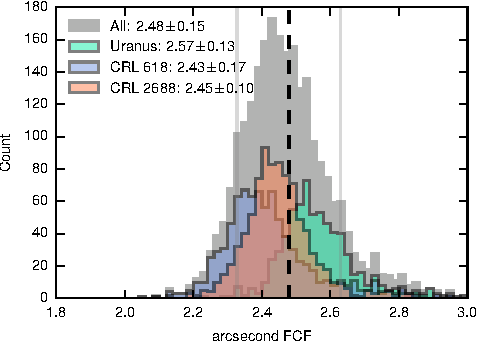
\includegraphics{lrvalues-histo}
  \caption{Histogram of FCFs, both for all sources (light gray) and
    separately for each source. The derived average FCF is shown as
    the dashed vertical line, with the $\pm$1s.d. shown as the light
    gray lines to either side.}
  \label{fig:calibhist}
\end{figure}

The co-adds in this release were calibrated using this mean FCF.  This
standard deviation represents a 1-$\sigma$ uncertainty of
approximately 6 percent. All co-adds were calibrated using the same
FCF. If it is wished to undo the calibration and redo with a different
value, please simply divide the data set by this FCF, and then
recalibrate using the FCF of your choice. Similarly, this can be done
with any flux values quoted in the catalogues derived from the
co-adds.%  A PICARD recipe (SCUBA2\_UNCALIBRATE\_DATA\footnote{see
% \url{http://www.starlink.ac.uk/cgi-bin/htxserver/sun265.htx/sun265.html?xref_SCUBA2_UNCALIBRATE_DATA}})
% is also provided as a convenience -- this will set the appropriate
% units within the data set.

For comparison, the usual `canonical' 850\,\micron\ arcsecond FCF used
in the JCMT's nightly reductions is $2.34 \pm 0.08 \mathrm{Jy}\
\mathrm{pW}^{-1}\ \mathrm{arcsec}^{-2}$ \citep{Dempsey2013}. This is
approximately 6 percent lower than the value used here, and was
derived using the `bright compact' \texttt{makemap} configuration on 1
arcsecond pixels (in comparison with the 3.22$\times$3.22 arcsecond
pixels in this release), using observations taken from 2011 to
20XX. Fig.\,\ref{fig:lr-caldb-histo} shows the comparison between the
histograms of bright compact derived FCFs and the legacy release
derived histogram, for the same
observations. Fig.\,\ref{fig:lr-caldb-scatter} shows the scatter plot
of each bright compact FCF vs the legacy release FCF for each
observation. Broadly speaking, we see an approximately linear
relationship between the two derivations of FCF.

\begin{figure}
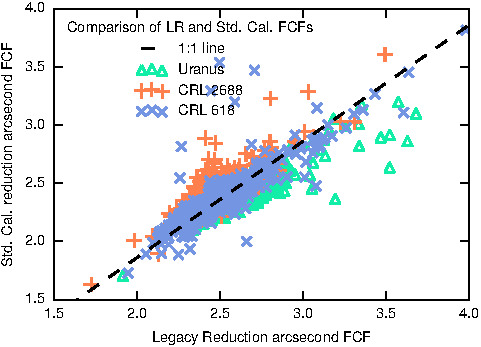
\includegraphics{legacyFCF-caldbFCF-scatter.pdf}
\caption{Comparison between the FCFs derived from the legacy release
  reductions, and those derived from the standard JCMT SCUBA-2
  calibrator reduction. The dashed line indicates a one-to-one
  relationship, offset by the difference in the derived FCF used for
  calibrating the legacy release (2.48) and the canonical FCF from
  \citet[2.34]{Dempsey2013}. \label{fig:lr-caldb-scatter} }
\end{figure}


To show the variation seen in the individual FCFs, we provide for
reference plots of the histogram of the FCFs
(Fig.~\ref{fig:calibhist}), the variation in FCF with opacity
(Fig.~\ref{fig:calibvstrans}) and the variation in FCF with date
(Fig.~\ref{fig:calibvstime}). No correction to the FCF for sky opacity or date
was made in this release.

\begin{figure}
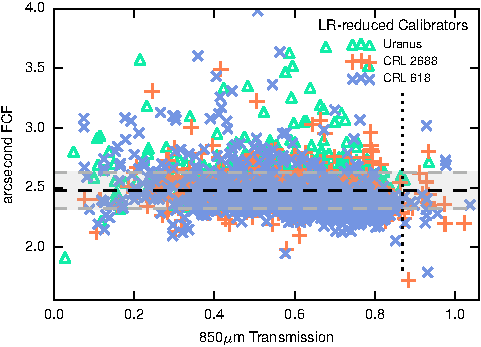
\includegraphics{legacyFCF-vs-transmission.pdf}
\caption{The legacy arcsecond FCFs derived from CRL 618, CRL 2688 and
  Uranus, shown against the 850\micron\ atmospheric transmission
  during the observation. Horizontal lines indicate the derived mean
  and standard deviation of the FCFs.\label{fig:calibvstrans}}
\end{figure}


\subsection{Uncertainty}

The standard deviation of the sample of derived FCFs represents the
minimum uncertainty in this calibration. In addition, we should take
into account the standard error in the sub-mm flux of
Uranus. \citet{Dempsey2013} quote this as $\pm$ 5 percent. Taken
together in quadrature, this gives an overall estimated error of
$\pm$8 percent.



% \section{Noise}

% % co-adds contain 1.69 gigapixels of non bad data.
% %
% \begin{itemize}
% \item Noise maps: overlaps work fine, show an example?
% \item Copy COHRS pixel distribution graph?
% \item noise on each pixel, noise vs integration time.
% \item High noise towards bright sources.
% \end{itemize}




%Noise vs integration time
% this is harder to do -- how to do a scatter plot of with billions of
% points.. 2-d histogram instead? produce in same way as the noise
% co-adds.

% Anomalous variance array values towards bright sources USe OMC-1 and
% cRL 618 as examples? Also visible in G34.3 shown earlier. Mentioned
% earlier.

\section{Pointing}
\begin{figure}
  \centering
  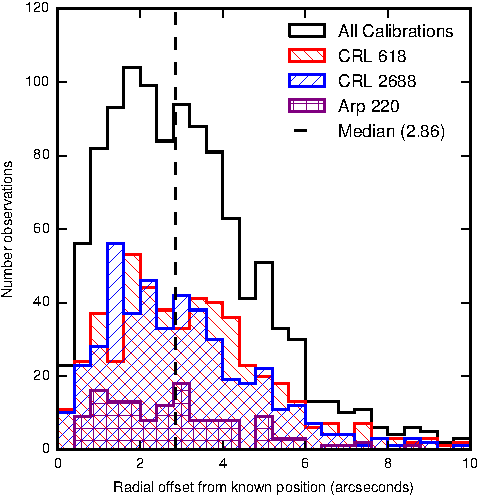
\includegraphics{pointing-offsets-by-source.pdf}
  \caption{Histogram of the total magnitude of the position offsets
    found in the JCMT Calibrator sources, with the three most-common
    sources shown separately. The median value of 2.86\arcsec{} is
    indicated on the plot. Note that a small number of observations
    with anomalously high values are not shown in the plot, although
    they were not cropped before calculating the median.}
  \label{fig:pointing}
\end{figure}

% explain the position fudging done for the calibration sources.
Our observations of JCMT standard calibrators and pointing sources are
corrected for normal pointing offsets, as these sources are all at
known positions. In our data reduction stage, these observations are
run through \texttt{makemap} twice; first to calculate the difference between
the beam position and the known source position, and secondly
re-reduced using this positional offset to place the observation at
the correct point. No other observations in this data set were
corrected for their positions.


The JCMT usually quotes a pointing offset of apporixmately 2\arcsec{}
in x and y, corresponding to an average radial offset of
2.9\arcsec{}. By examining the offsets in x and y found for the
calibrator observations, we identified that the average offset for the
calibrators in this release matches this expected value, with a median
radial offset of 2.86\arcsec{}. See Figure~\ref{fig:pointing} for the
histogram of these sources. We assume that the pointing in our
non-calibration observations should follow the same distribution. \note{When
comparing normal observations to the beam shapes of the
pointing-corrected co-adds, a correction factor of 2.9\arcsec\ beam
smearing should be included in the resolution.}
\note{Get citation for JCMT expected average pointing issue. Probably
  website?}

\note{TODO: add in images and cut throughs of CRL618 and CRL2688
  beams, with Gaussian fits. Similar to Jess's calibration paper, but
  a little less thorough?}

%\end{itemize}





\section{Conclusions}
\note{do we need a conclusion section?}

\acknowledgments
The James Clerk Maxwell Telescope has historically been operated by
the Joint Astronomy Centre on behalf of the Science and Technology
Facilities Council of the United Kingdom, the National Research
Council of Canada and the Netherlands Organisation for Scientific
Research. This work was funded by the Science and Technology
Facilities Council.  Additional funds for the construction of SCUBA-2
were provided by the Canada Foundation for Innovation.

The work presented here was initially started by the Joint Astronomy
Centre, and latterly has been supported by East Asian Observatory (EAO).
EAO operates the JCMT since 2015 March 1, on behalf of The
National Astronomical Observatory of Japan, Academia Sinica Institute
of Astronomy and Astrophysics, the Korea Astronomy and Space Science
Institute, the National Astronomical Observatories of China and the
Chinese Academy of Sciences (Grant No. XDB09000000), with additional
funding support from the Science and Technology Facilities Council of
the United Kingdom and participating universities in the United
Kingdom and Canada.

This research used the facilities of the Canadian Astronomy Data
Centre operated by the National Research Council of Canada with the
support of the Canadian Space Agency.
\vspace{5mm}
\facility{JCMT(SCUBA-2)}
% Comma separated list, include software citations here as \citep{}
% after name of software, before next comma.Should this
% include astropy? It was used for analysis and figures.
\software{Starlink \citep{starlink?}, SMURF, KAPPA, ORAC-DR}



\bibliography{legacy-850um-paper}
\bibstyle{aasjournal.bst}




\clearpage
\appendix


%% Probably more detailed than needed in a paper
\section{Mapmaker configuration}
\label{app:config}
The mapmaker configuration used for this release (known as a
\texttt{dimmconfig}) is shown here. Like most SCUBA-2 mapmaker
configuration files, it first sources the \emph{base}
\texttt{dimmconfig} file that sets up the basic values for a range of
options and then tweaks a subset of additional parameters or its
purposes. This file is shipped in the 2015A Starlink release. The
value of every configuration parameter used is written into the
history component of the file.

\begin{verbatim}
^$STARLINK_DIR/share/smurf/dimmconfig.lis

#  Less aggressive cleaning to cope with bright sources
noisecliphigh=10.0
dcthresh = 100

#  Don't want extended structure, so avoid problems with COM model by using
#  individual common-mode models for each subarray.
com.perarray = 1

#  Aggressive filtering.
flt.filt_edge_largescale=200

#  Allow bolometer noise to vary with time, and using a box filter to
#  determine mean noise in each box, in order to presevre as many samples
#  as possible.
noi.box_size=-15
noi.box_type=1

#  Use a maximum of 20 iterations
numiter=-25
maptol_mean=1
maptol=0.01

# new recommendations and using an ast model
ast.zero_snr = 5
ast.zero_snrlo = 3

ast.skip=5
flt.zero_snr=5
flt.zero_snrlo=3
\end{verbatim}




%\newpage

\onecolumngrid
\section{Full listing of file types in this release}
\begin{deluxetable}{llp{4.5cm}p{3.5cm}p{3.5cm}l}
\floattable
\tabletypesize{\scriptsize}
\tablewidth{\linewidth}
\rotate
\tablecolumns{7}
\tablecaption{Listing of all types files contained in this data release.}
\tablehead{\colhead{Object} & \colhead{recipe} & \colhead{filename} & \colhead{Contained in file} & \colhead{Notes} & \colhead{productID}}
\startdata
Single observation
& \multicolumn{1}{p{2.5cm}}{REDUCE\_SCAN\_JSA\_PUBLIC}
& \texttt{jcmts<YYYYMMDD>\_<scan>\_850\_healpix<TILE>_obs_000.fits}&
\raggedright{\textbullet{} Emission map (pW)}\linebreak
\raggedright{\textbullet{} Variance map (pW\textsuperscript{2})}\linebreak
\raggedright{\textbullet{} Quality map (mask)}
& Multiple files per observation, one for each tile the observation fell onto & healpix-850um\\
%
Co-added tile &  COADD\_JSA\_TILES  & \texttt{jcmts850um\_healpix<TILE>\_pub\_001.fits} &
\raggedright{\textbullet{} Emission map (m\jyas)}\linebreak
\raggedright{\textbullet{} Variance map (m\jyas)\textsuperscript{2}}
 & One file per tile & healpix-850um\\
%
Extent catalog & JSA\_CATALOGUE&\texttt{jcmts850um\_extent-cat<TILE>\_pub\_001.fits}
&\textbullet{} Catalog for extents (see Sec.\,\ref{sec:extents})
& Only created if  emission detected at $>5\sigma$. & extent-850um\\
%
Extent mask & JSA\_CATALOGUE & \texttt{jcmts850um_extent-mask<TILE>\_pub\_001.fits} &
\textbullet{}Mask map indicating which pixels fell into which extent
& " & "\\
%
Extent MOC & JSA\_CATALOGUE & \texttt{jcmts850um\_extent-moc<TILE>\_pub\_001.fits} &
\textbullet{}MOC file, indicating which pixels fell into any extent & " & "\\
Peak catalog & JSA\_CATALOGUE & \texttt{jcmts850um\_peak-cat<TILE>\_pub\_001.fits} &
\textbullet{}Catalog of peaks (see Sec.\,\ref{sec:peaks})&
Only created if extents catalog created. & peak-850um\\
Peak MOC & JSA\_CATALOGUE & \texttt{jcmts850um\_peak-moc<TILE>\_pub\_001.fits} &
\textbullet{}MOC file, indicating which pixels were as a identified.& " & "\\
Coverage MOC & JSA\_CATALOGUE & \texttt{jcmts850um\_tile-moc<TILE>\_pub\_001.fits} &
\textbullet{}MOC file, identifying all pixels which contain a valid data point (as opposed to blank regions of tile) & Created for all tiles. & extent-850um\\
\enddata
\tablecomments{In the filename column, \texttt{<SCAN>} indicates the
  JCMT scan number of that observation, padded with zeros to five-digit
  length. \texttt{<YYYYMMDD>} indicates the UT date of the
  observation. \texttt{<TILE>} indicates the HEALPix tile number of
  that tile, using the nested scheme and the HEALPix parameters given
  in Table\,\ref{tab:hpxpar}.
  \\
  The \emph{single observation} files will be found in the JSA under the
  original observations metadata, obsid and project code. All
  remaining files are in the JSA in a tile-centric fashion, and are found under the project
  code 'JCMT-LR', with metadata appropriate for the specific tile, and
  with an obsid of the form \texttt{SCUBA-2-<TILE>}.}
\end{deluxetable}

\section{Example Catalogs}
For guidance, excerpts from the extent and peak catalogs of tile 30318
are shown here.
\begin{deluxetable}{c c c c c c p{7cm}}
\tablecaption{An excerpt from the catalog of extents for Tile 30318.\label{tab:extents}}
\tablehead{\colhead{ID} & \colhead{RA} & \colhead{DEC} & \colhead{TOTAL_FLUX} & \colhead{PEAK_FLUX} & \colhead{AREA} & \colhead{SHAPE}\\ \colhead{ } & \colhead{deg} & \colhead{deg} & \colhead{$\mathrm{mJy}$} & \colhead{mJy\,arcsec$^{-2}$} & \colhead{arcsec$^{-2}$} & \colhead{ }}
\startdata
JCMTPX_J185318.8+011459 & 283.3285 & 1.2497 & 5.415E+09 & 2.105E+02 & 1.633E+05 & Polygon ICRS TOPOCENTER 283.3003 1.256714 283.2408 1.289357 283.3113 1.273799 283.3003 1.308009 283.3347 1.306843 283.3283 1.386135 283.3019 1.392549 283.3381 1.488935 283.3406 1.306847 283.3964 1.189091 283.3532 1.215324 283.3594 1.166936 283.3271 1.152366 283.339 1.196665 283.2928 1.201333 \\
JCMTPX_J185334.7+011421 & 283.3944 & 1.2392 & 2.599E+06 & 1.647E+00 & 8.609E+03 & Polygon ICRS TOPOCENTER 283.3889 1.235147 283.3855 1.240392 283.3759 1.241558 283.3841 1.256706 283.3878 1.257872 283.391 1.268366 283.3944 1.268947 283.3958 1.260787 283.4051 1.254378 283.3996 1.246216 283.4026 1.238634 283.4102 1.231055 283.4109 1.222318 283.4074 1.221737 283.4061 1.226401 \\
JCMTPX_J185330.0+010240 & 283.3752 & 1.0445 & 5.236E+06 & 5.745E+00 & 7.148E+03 & Polygon ICRS TOPOCENTER 283.3608 1.032857 283.3603 1.036351 283.3624 1.039264 283.3612 1.04218 283.3621 1.049172 283.369 1.051884 283.3841 1.050334 283.3866 1.046261 283.3845 1.039849 283.3871 1.035768 283.3848 1.034608 283.382 1.029943 283.3738 1.023732 283.3669 1.029947 283.3635 1.030529 \\
JCMTPX_J185322.6+010831 & 283.3443 & 1.1419 & 2.774E+05 & 9.040E-01 & 2.702E+03 & Polygon ICRS TOPOCENTER 283.3363 1.137201 283.3392 1.141282 283.3408 1.148856 283.3491 1.15235 283.3518 1.150022 283.3523 1.147694 283.347 1.13429 283.3436 1.131768 283.3367 1.135266 \\
JCMTPX_J185321.5+010610 & 283.3395 & 1.1028 & 7.271E+05 & 1.185E+00 & 4.310E+03 & Polygon ICRS TOPOCENTER 283.3337 1.100475 283.3335 1.105721 283.3351 1.109802 283.3321 1.117381 283.3367 1.122421 283.3388 1.121457 283.339 1.117381 283.3461 1.102807 283.3468 1.098726 283.3447 1.094645 283.3472 1.088237 283.3381 1.083192 283.3347 1.085322 283.3347 1.088812 283.3392 1.09348
\enddata
\end{deluxetable}

\begin{deluxetable}{ccccc}
\tablecaption{An excerpt from the catalog of peaks for Tile 30318.\label{tab:peaks}}
\tablehead{\colhead{ID} & \colhead{RA} & \colhead{DEC} & \colhead{PEAK_FLUX} & \colhead{PARENT_EXTENT}\\ \colhead{ } & \colhead{deg} & \colhead{deg} & \colhead{mJy\,arcsec$^{-2}$} & \colhead{ }}
\startdata
JCMTPP_J185318.8+011459 & 283.3285 & 1.2497 & 2.105E+02 & JCMTPX_J185318.8+011459 \\
JCMTPP_J185318.2+012524 & 283.3257 & 1.4234 & 4.608E+01 & JCMTPX_J185318.8+011459 \\
JCMTPP_J185316.0+011518 & 283.3168 & 1.2550 & 3.018E+01 & JCMTPX_J185318.8+011459 \\
JCMTPP_J185318.7+012445 & 283.3278 & 1.4124 & 2.470E+01 & JCMTPX_J185318.8+011459 \\
JCMTPP_J185316.5+011434 & 283.3189 & 1.2427 & 2.004E+01 & JCMTPX_J185318.8+011459 \\
JCMTPP_J185321.6+011341 & 283.3401 & 1.2281 & 1.224E+01 & JCMTPX_J185318.8+011459 \\
JCMTPP_J185320.8+012825 & 283.3367 & 1.4736 & 7.523E+00 & JCMTPX_J185318.8+011459 \\
JCMTPP_J185319.8+011257 & 283.3326 & 1.2159 & 5.712E+00 & JCMTPX_J185318.8+011459 \\
JCMTPP_J185315.2+011713 & 283.3134 & 1.2870 & 4.566E+00 & JCMTPX_J185318.8+011459 \\
JCMTPP_J185318.2+011339 & 283.3257 & 1.2276 & 2.932E+00 & JCMTPX_J185318.8+011459 \\
JCMTPP_J185316.9+011318 & 283.3202 & 1.2217 & 2.896E+00 & JCMTPX_J185318.8+011459 \\
JCMTPP_J185328.2+011350 & 283.3676 & 1.2305 & 2.699E+00 & JCMTPX_J185318.8+011459 \\
JCMTPP_J185322.5+011211 & 283.3436 & 1.2031 & 2.474E+00 & JCMTPX_J185318.8+011459 \\
JCMTPP_J185326.9+011251 & 283.3621 & 1.2142 & 2.456E+00 & JCMTPX_J185318.8+011459 \\
JCMTPP_J185323.4+011137 & 283.3477 & 1.1937 & 2.224E+00 & JCMTPX_J185318.8+011459 \\
JCMTPP_J185324.3+011119 & 283.3511 & 1.1885 & 2.164E+00 & JCMTPX_J185318.8+011459 \\
JCMTPP_J185320.5+012224 & 283.3353 & 1.3733 & 2.119E+00 & JCMTPX_J185318.8+011459 \\
JCMTPP_J185307.1+011600 & 283.2797 & 1.2666 & 2.098E+00 & JCMTPX_J185318.8+011459 \\
JCMTPP_J185318.2+012722 & 283.3257 & 1.4561 & 2.053E+00 & JCMTPX_J185318.8+011459 \\
JCMTPP_J185326.9+011551 & 283.3621 & 1.2643 & 1.935E+00 & JCMTPX_J185318.8+011459 \\
JCMTPP_J185325.4+011318 & 283.3559 & 1.2217 & 1.769E+00 & JCMTPX_J185318.8+011459 \\
JCMTPP_J185319.2+012653 & 283.3298 & 1.4479 & 1.654E+00 & JCMTPX_J185318.8+011459 \\
JCMTPP_J185311.4+011617 & 283.2976 & 1.2713 & 1.638E+00 & JCMTPX_J185318.8+011459 \\
JCMTPP_J185316.7+012629 & 283.3195 & 1.4415 & 1.546E+00 & JCMTPX_J185318.8+011459 \\
JCMTPP_J185323.8+011047 & 283.3491 & 1.1798 & 1.528E+00 & JCMTPX_J185318.8+011459 \\
JCMTPP_J185316.7+011638 & 283.3195 & 1.2771 & 1.292E+00 & JCMTPX_J185318.8+011459 \\
JCMTPP_J185305.3+011549 & 283.2722 & 1.2637 & 1.278E+00 & JCMTPX_J185318.8+011459 \\
JCMTPP_J185320.5+012043 & 283.3353 & 1.3453 & 1.212E+00 & JCMTPX_J185318.8+011459 \\
JCMTPP_J185318.2+011623 & 283.3257 & 1.2730 & 1.204E+00 & JCMTPX_J185318.8+011459 \\
JCMTPP_J185320.3+011921 & 283.3347 & 1.3226 & 1.091E+00 & JCMTPX_J185318.8+011459 \\
JCMTPP_J185325.9+011407 & 283.3580 & 1.2351 & 9.760E-01 & JCMTPX_J185318.8+011459 \\
JCMTPP_J185321.5+012657 & 283.3395 & 1.4491 & 9.413E-01 & JCMTPX_J185318.8+011459 \\
JCMTPP_J185313.2+011253 & 283.3051 & 1.2147 & 9.409E-01 & JCMTPX_J185318.8+011459 \\
JCMTPP_J185312.2+011318 & 283.3010 & 1.2217 & 8.789E-01 & JCMTPX_J185318.8+011459 \\
JCMTPP_J185323.1+011421 & 283.3463 & 1.2392 & 8.282E-01 & JCMTPX_J185318.8+011459 \\
JCMTPP_J185319.3+011003 & 283.3305 & 1.1675 & 8.077E-01 & JCMTPX_J185318.8+011459 \\
JCMTPP_J185313.4+012333 & 283.3058 & 1.3925 & 7.729E-01 & JCMTPX_J185318.8+011459 \\
JCMTPP_J185315.7+012329 & 283.3154 & 1.3914 & 7.310E-01 & JCMTPX_J185318.8+011459 \\
JCMTPP_J185330.2+011243 & 283.3759 & 1.2118 & 7.295E-01 & JCMTPX_J185318.8+011459 \\
JCMTPP_J185305.0+011726 & 283.2708 & 1.2905 & 6.510E-01 & JCMTPX_J185318.8+011459\\
\enddata
\end{deluxetable}


\newpage
\section{Extra images}
These will probably be removed.
\begin{figure*}[h!]
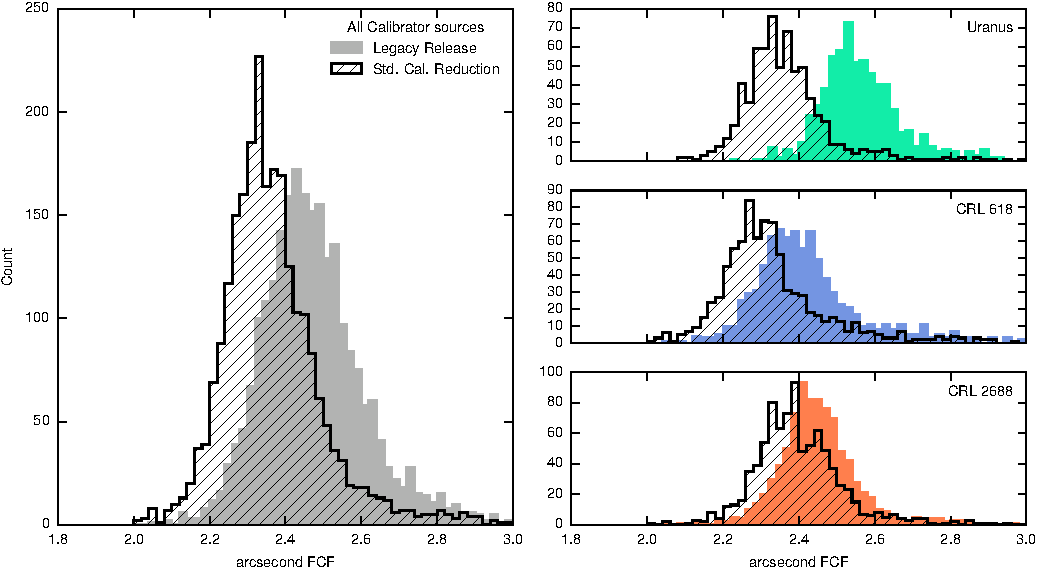
\includegraphics{legacyFCF-caldbFCF-histograms.pdf}
\caption{Comparison between the histograms of
  arcsecond FCFs derived from the legacy reduction and the standard
  JCMT SCUBA-2 calibrator reduction, for the same observations.
  These are shown both overall and broken down by source (CRL 618,
  CRL 2688 and Uranus). Note that the LR Uranus maps were \emph{not}
  reduced onto a Healpix grid, but did use the same pixel area and
  \texttt{makemap} dimmconfig as the other LR reductions.\label{fig:lr-caldb-histo}}
\end{figure*}

\begin{figure*}
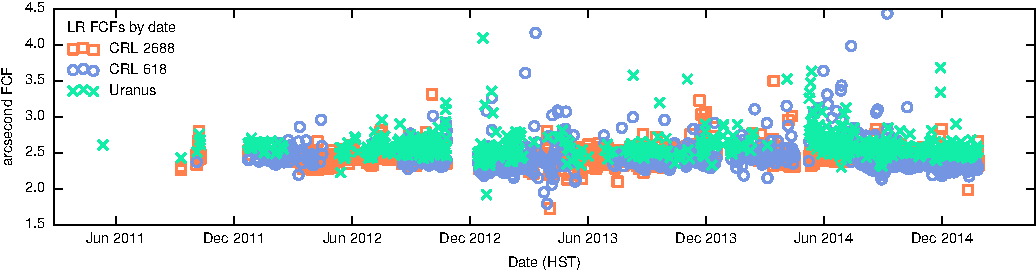
\includegraphics{legacyFCF-vs-date.pdf}
\caption{The arcsecond FCFs derived for the legacy reductions of CRL
  618, CRL 2688 and Uranus, shown against time. Although there is a
  large scatter and some hints of variation , it can be seen that there is not
  clear overall dependency with time.\label{fig:calibvstime}}
\end{figure*}

\end{document}
